\documentclass[a4paper, twoside]{report}

%% Language and font encodings
\usepackage[english]{babel}
\usepackage[utf8x]{inputenc}
\usepackage[T1]{fontenc}

%% Sets page size and margins
\usepackage[a4paper,top=3cm,bottom=2cm,left=3cm,right=3cm,marginparwidth=1.75cm]{geometry}

%% Useful packages
\usepackage[hyphens]{url}
\usepackage[colorlinks=true, allcolors=blue]{hyperref}
\usepackage{multirow}
\usepackage{amsmath}
\usepackage{graphicx}

\setlength{\marginparwidth}{2cm}
\usepackage[colorinlistoftodos]{todonotes}

% adds newline, removes autoindent for new paragraphs
\usepackage{parskip}

% Remove extra spacing in itemize and enumerate
\usepackage{enumitem}
\setlist{nosep}

% allows tables to be centred when going past text margins
\usepackage{adjustbox}

% increase height of each row in table relative to default height
\renewcommand{\arraystretch}{1.2}

% typesetting algorithms
\usepackage{algorithm} 
\usepackage{algpseudocode}

% use subfigures
\usepackage{subcaption}

% checks for unused references
%\usepackage{refcheck}

\title{Detecting Political Bias On Social Media With Improved Domain Adaptation Techniques}
\author{Fawaz Shah}
% Update supervisor and other title stuff in title/title.tex

\begin{document}
\begin{titlepage}

\newcommand{\HRule}{\rule{\linewidth}{0.5mm}} % Defines a new command for the horizontal lines, change thickness here

%----------------------------------------------------------------------------------------
%	LOGO SECTION
%----------------------------------------------------------------------------------------


\includegraphics[width=8cm]{0-title/logo.eps}\\[1cm] % Include a department/university logo - this will require the graphicx package
 
%----------------------------------------------------------------------------------------

\center % Center everything on the page

%----------------------------------------------------------------------------------------
%	HEADING SECTIONS
%----------------------------------------------------------------------------------------

\textsc{\LARGE MEng Individual Project}\\[1.5cm] % Name of your university/college
\textsc{\Large Imperial College London}\\[0.5cm] % Major heading such as course name
\textsc{\large Department of Computing}\\[0.5cm] % Minor heading such as course title

%----------------------------------------------------------------------------------------
%	TITLE SECTION
%----------------------------------------------------------------------------------------
\makeatletter
\HRule \\[0.6cm]
{ \huge \bfseries \@title}\\[0.3cm] % Title of your document
\HRule \\[1.5cm]
 
%----------------------------------------------------------------------------------------
%	AUTHOR SECTION
%----------------------------------------------------------------------------------------

\begin{minipage}{0.4\textwidth}
\begin{flushleft} \large
\emph{Author:}\\
\@author % Your name
\end{flushleft}
\end{minipage}
~
\begin{minipage}{0.4\textwidth}
\begin{flushright} \large
\emph{Supervisor:} \\
Dr Anandha Gopalan \\[1.2em] % Supervisor's Name
\emph{Second Marker:} \\
Dr Francesco Belardinelli % second marker's name
\end{flushright}
\end{minipage}\\[2cm]
\makeatother

% If you don't want a supervisor, uncomment the two lines below and remove the section above
%\Large \emph{Author:}\\
%John \textsc{Smith}\\[3cm] % Your name

%----------------------------------------------------------------------------------------
%	DATE SECTION
%----------------------------------------------------------------------------------------

{\large \today}\\[2cm] % Date, change the \today to a set date if you want to be precise

\vfill % Fill the rest of the page with whitespace

\end{titlepage}

\begin{abstract}

\end{abstract}

\renewcommand{\abstractname}{Acknowledgements}
\begin{abstract}

\end{abstract}

\tableofcontents
\listoffigures
\listoftables

\chapter{Introduction}

Biases play a huge role in how we perceive and react to media. There are many documented types of media bias that exist \cite{types-of-bias}, including temporal bias (bias towards events that are happening today), bad-news bias, and many more. In this project we focus on political bias.

Political bias is being increasingly scrutinised in the modern-day media. The presence of political bias in the media isn't new - newspapers have pledged their allegiances to particular political parties since the 19th and early 20th centuries \cite{partisanship-history} - however there has also been a big shift in the last 30 years from objective news to more subjective, opinionated reporting \cite{subjective-news}. Regardless, there is a global appetite for unbiased news: a Pew Research survey found that across 38 countries 75\% of participants said it is not acceptable for a news organisation to favour one political party over another \cite{pew-unbiased}, although only 52\% thought that their own country's news media report different positions on political issues fairly.

Social media usage has soared in the last decade, with the largest social networks sporting billions of users \cite{rise-of-social-media}, leading to a dramatic rise in the number of people getting their news from social media. The Pew Research Center found in 2018 that 68\% of Americans get their news from social media \cite{pew-social-media-news-2018}, and that Facebook, Twitter and Reddit were the sites on which the highest proportion of users were exposed to news.

Detecting political bias in the news is a key problem being tackled today, but a relevant side-problem is identifying \textit{readership bias} - the biases of those who read the news, and exploring how audiences react to modern media. Readership bias is a highly under-explored area in literature - it is hard to find any examples of people's reactions to particular news being analysed. Improved political bias detection on social media will help us understand readership bias, and help us tackle further problems on social media such as filter bubbles and echo chambers.

Work has already been done to manually classify news sources by political bias, such as by Media Bias/Fact Check \cite{mbfc} and Ad Fontes Media \cite{media-bias-chart}, however detecting any bias manually comes with several problems. Volunteers often need an education in political science and/or bias detection training before they can label biased text, and volunteers may also bring their own internal political bias to their labelling. We therefore consider applying machine learning and natural language processing techniques to these problems. Machine learning models only examine characteristics of the language itself, without any preconceived notions of politics or the current political atmosphere, and once trained a model can be quickly deployed for inference on any amount of new text, significantly speeding up the bias detection process.

Examining social media content for bias presents a different textual `domain' to news article text. We therefore aim to explore and extend state-of-the-art domain adaptation methods with the goal of improving bias detection on social media.

main objectives

 - survey existing methods for detecting political bias
 
 - explore transfer learning, specifically domain adaptation, as a way to improve accuracy of detecting readership bias on social media

\section{Contributions}

The main contributions of this dissertation are as follows:

\begin{itemize}
    \item \textbf{Detecting political bias with ensemble classifiers and BERT} - We survey existing machine learning models for detecting political bias, including ensemble classifiers that have not been explored in prior literature. We assess performance using pre-computed features from previous research, as well as using models such as BERT that perform textual feature extraction themselves. See Chapter \ref{chap:ensemble-bert}.
    \item \textbf{Developing a cross-domain Reddit dataset} - We create a novel dataset consisting of both news articles and Reddit comments that address those articles, aimed at domain adaptation tasks. We discuss the design decisions and trade-offs involved in creating a high-quality dataset, and assess similarity between the domains in our dataset. See Chapter \ref{chap:reddit-data}.
    \item \textbf{Exploring and extending unsupervised domain adaptation} - We investigate unsupervised domain adaptation to detect political bias on Reddit, and extend a state-of-the-art domain-adaptive BERT model, yielding a 3\% increase in accuracy on this task. See Chapter \ref{chap:domain-adaptation}.
\end{itemize}

\chapter{Background}

In this chapter we cover several elements of background research needed for the project. We introduce the idea of political bias (Section \ref{sec:political-bias}), and look at existing datasets of news content annotated by political bias (Section \ref{sec:existing-datasets}), followed by machine learning methods that have been employed to detect bias in news (Section \ref{sec:detecting-political-bias-in-news}). We then introduce Reddit (Section \ref{sec:reddit}) and the idea of readership bias (Section \ref{sec:readership-bias}), and explore related work in detecting readership bias on social media. Finally, we introduce transfer learning (Section \ref{sec:transfer-learning}) and specifically previous work in domain adaptation (Section \ref{subsec:domain-adaptation}).

\section{Political bias} \label{sec:political-bias}

Discussions on political bias are mainly focused on whether a particular news source is left-wing or right-wing. The definition of each is not clear-cut, and the boundaries between what constitutes left-wing thought and right-wing thought varies between countries, and between historical periods and today.

A YouGov survey \cite{yougov} in 2019 found that issues in the UK that matter most to left-wing voters include remaining in the EU, opposing the use of nuclear weapons, increasing the minimum wage, supporting industry nationalisation and increasing wealth tax, whereas right-wing voters support the opposite viewpoint. In the USA \cite{diffen} left-wing viewpoints include expanding government healthcare programs and social security, tightening environmental regulation, increasing corporation tax, expanding amnesty to undocumented immigrants, and again right-wing viewpoints are in opposition.

Overarching themes that can be drawn include that left-wing thought more often than not supports expanding the role of government, whereas right-wing thought advocates for smaller government. Economically, left wing voters tend to support tight financial regulation, however right wing voters support less regulation in favour of a free market economy, and left wing voters often support globalisation and stronger international ties with other countries whereas right wing voters are more sceptical of globalisation and may prefer protectionism.

Of course, political bias in text can be extremely nuanced, hence the interest in using automatic natural language processing methods for detection.

\section{Existing datasets} \label{sec:existing-datasets}

In this section we look at some existing datasets of news sources and news articles that have been annotated by political bias.

\subsection{Media Bias/Fact Check}

Media Bias/Fact Check (MBFC) provides a list of over 3500 news sources, annotated with their respective political bias leanings \cite{mbfc}. The news sources covered are mostly US-based, and include mainstream and non-mainstream media - examples include CNN, Fox News, Breitbart, Bloomberg, and many more.

MBFC has a team of volunteers who manually assess and assign scores per-source based on content from their articles. Each source is scored from 1-10 on the four following categories: biased wording/headlines, factuality/well-sourced information, story portrayal, and political affiliation \cite{MBFC-methodology}. The scoring mechanism is shown in Table \ref{tab:MBFC-scoring}.

\begin{table}[ht]
    \centering
    \begin{tabular}{|c|c|c|c|}
        \hline
        0-2 & 2-5 & 5-8 & 8-10 \\
        \hline
        Least Biased & Slightly Biased & Moderately Biased & Extremely Biased \\
        \hline
    \end{tabular}
    \caption{MBFC scoring mechanism}
    \label{tab:MBFC-scoring}
\end{table}

The scores across the 4 categories are averaged to produce an overall score for each news source. Note that this scale only measures the degree of bias and not the direction of bias (e.g. left/right wing) - this is manually classified by MBFC's volunteers. MBFC also produces a detailed report giving more information about each source's particular traits, for example the following is a sample from the report on CNN:

\begin{quote}
\textit{``...we rate CNN left biased based on editorial positions that consistently favors the left, while straight news reporting falls left-center through bias by omission. We also rate them Mixed for factual reporting due to several failed fact checks by TV hosts. However, news reporting on the website tends to be properly sourced with minimal failed fact checks.''} \cite{MBFC-CNN}
\end{quote}

Note since most catalogued news sources are based in the USA, this scale is centred heavily on the US political scale.

\subsection{News-Media-Reliability} \label{subsec:news-media-reliability}

Baly et al., as part of their analysis on detecting political bias \cite{baly-emnlp18}, created the News-Media-Reliability dataset \cite{news-media-reliability}, a collection of engineered features from 1066 news sites, with political bias annotations provided by Media Bias/Fact Check. Sites are categorised according to 7 labels: \textit{extreme-left, left, center-left, center, center-right, right} and \textit{extreme-right}. The dataset features include textual features from each site's article content and its headlines, as well as information from the site's Twitter page and Wikipedia page (if they exist), and its Alexa web traffic rank. The full collection of features is given in Table \ref{tab:nmr-features}.

\begin{table}[h!]
    \centering
    \begin{tabular}{|c|c|c|}
        \hline
        \textbf{Category} & \textbf{Feature} & \textbf{Description} \\
        \hline
        Site traffic & alexa & Alexa ranking \\
        \hline
        URL & url\_structure & Site URL \\
        \hline
        \multirow{2}{4em}{Articles} & articles\_title\_glove & Article headline features \\
        & articles\_body\_glove & Article body features \\
        \hline
        \multirow{7}{4em}{Twitter} & has\_twitter & Whether site has Twitter or not \\
        & twitter\_created\_at & Year Twitter account was created \\
        & twitter\_description & Twitter account biography \\
        & twitter\_engagement & Twitter user engagement metrics \\
        & twitter\_haslocation & Whether site has location in their Twitter biography or not \\
        & twitter\_urlmatch & Whether Twitter account contains a link to the site URL \\
        & twitter\_verified & Whether Twitter account is verified or not \\
        \hline
        \multirow{4}{4em}{Wikipedia} & wikipedia\_categories & Wikipedia page categories features \\
        & wikipedia\_content & Wikipedia page content features \\
        & wikipedia\_summary & Wikipedia page summary features \\
        & wikipedia\_toc &  Wikipedia page table of contents features \\
        \hline
    \end{tabular}
    \caption{Engineered features in the News-Media-Reliability dataset}
    \label{tab:nmr-features}
\end{table}

The articles\_title\_glove and articles\_body\_glove features aren't actually the text content of the headline/body, but a set of 141-dimensional custom features relating to the structure of the text, sentiment scores, language bias analysis and also complexity of the text, expressed as 141-vectors. More details are given in Baly et al. \cite{baly-emnlp18}. The Wikipedia features are word2vec word embeddings of the corresponding text (see Section \ref{subsec:word-embeddings} for more detail). Overall this featureset is fairly comprehensive, as it includes a well-rounded representation of a news source's article content plus content taken from the source's online presence.

\section{Detecting political bias in the news} \label{sec:detecting-political-bias-in-news}

In this section we will look at examples of techniques that have been applied to detect political bias in the news with NLP.

\subsection{Word embeddings} \label{subsec:word-embeddings}

In order to run machine learning models on words, they must first be converted into feature vectors. Word embeddings are a representation of words in a finite-dimensional vector space, such that the word embeddings of words that are semantically similar are closer to each other in the vector space. Word embeddings can be learnt manually by training a neural network to generate them using an embedding layer, or pre-trained models can be used such as Google's word2vec \cite{word2vec}, or GloVe \cite{glove}.

Word embeddings by themselves have been used to analyse bias in text. Bolukbasi et al. \cite{gender-bias-word-embeddings} use the cosine similarity between averaged word embeddings of Google News articles to detect gender bias, and Gordon et al. \cite{political-bias-word-embeddings} use the same idea on tweets to detect political bias. However, they are most often used as a pre-processing technique for machine learning models.

\subsection{SVMs} \label{subsec:svms}

Support vector machines (SVMs) are supervised models that can be used for both classification and regression. In the classification case, finding the decision boundary between classes in feature space is formulated as an optimisation problem, which the classifier approximates using gradient descent. We can change the function being used to model the decision boundary, called the kernel. A common kernel used instead of the standard linear one is the radial basis function (RBF) kernel. This is useful for modelling classes which occur in spherical clusters rather than with straight-line boundaries.

Baly et al. \cite{baly-emnlp18} trained an SVM classifier to detect political bias in the News-Media-Reliability dataset. They used an RBF kernel, and provided F1 and accuracy scores for classifiers trained on individual News-Media-Reliability features (see Table \ref{tab:nmr-features}) as well as groups of features, compared to a `majority' baseline that always predicts the majority class in the dataset (i.e. the modal class). They achieved a highest F1 score of 61.31\% and accuracy of 68.86\% after merging small classes. The code and the dataset for this study are open-source and available on GitHub, making it easy to reproduce the paper's results. The authors do not compare SVMs with any other classifiers, providing ample opportunity for future work.

\subsection{Ensemble classifiers} \label{subsec:ensemble-classifiers}

Ensemble classifiers involve aggregating predictions from a group of classifiers, called \textit{base learners}, in order to improve accuracy when compared to individual classifiers. In the classification case, aggregation usually involves taking a majority vote from the base learners' predictions. In order for ensemble learning to work, the base learners should ideally be uncorrelated (that is, there shouldn't be any patterns between predictions of any two base learners for the same training samples).

Two common ensemble learning techniques are \textit{bagging} and \textit{boosting}. Bagging (\underline{B}ootstrap \underline{Agg}regating) involves bootstrapping say, $ T $ new training datasets from an original dataset, and training $ T $ independent base learners on each new dataset. During inference time, a majority vote of predictions from each base learner is used to form an overall prediction. A popular bagging technique is a random forest, which is a ensemble of decision trees.

Boosting involves training base learners serially on the same training set, instead of in parallel as with bagging. In Adaboost, the first boosting algorithm created, any mis-classified examples from one learner are upweighted for the next learner, meaning an ensemble of the base learners learns a good representation of all the data. Adaboost uses decision stumps as base learners (decision trees of depth 1). In a more modern technique called gradient-boosted trees, full decision trees are used as base learners, and residual errors from previous learners are factored in to each learner's training.

Ensemble classifiers have not been extensively explored for the problem of detecting political bias. Voong et al. \cite{voong} compared gradient-boosted forests to Naive Bayes classifiers, SVMs, and logistic regression in detecting political bias of tweets, finding gradient-boosted forests gave the highest accuracy and F1 scores.

\subsection{BERT}

BERT (Bidirectional Encoder Representations from Transformers) \cite{bert} is a transformer-based model developed for natural language processing purposes. Transformer networks can learn contexts across extremely long sentences and paragraphs, and also enables bi-directional training that allows transformers to learn context even more deeply.

BERT is a stack of encoder models that utilises semi-supervised learning. This means BERT models are often pre-trained for use with a particular language, e.g. English, and then fine-tuned for a particular NLP task. Fine-tuning is often fast, as the main bulk of training is performed in pre-training. Pre-training involves two tasks:
\begin{itemize}
    \item \textbf{Masked Language Modelling (MLM)} - random words in the input text are replaced with \texttt{[MASK]} tokens, and BERT is trained to predict the missing words. This helps BERT understand bi-directional context between words in a single sentence.
    \item \textbf{Next Sentence Prediction (NSP)} - BERT takes in two sentences A and B, and determines whether sentence B actually follows sentence A in the text or not. This helps BERT understand context across lots of sentences.
\end{itemize}

A diagram of BERT during both pre-training and fine-tuning is shown in Figure \ref{fig:bert-pretraining-finetuning}. During pre-training, BERT generates its own contextualised word embeddings which it then uses throughout the encoder stack. BERT models come in varying sizes, the most popular being `base' and `large'. The base model contains 12 layers with each hidden layer containing 768 neurons, and gives 110M trainable parameters overall. The large model contains 24 layers each with 1024 neurons, and gives 340M trainable parameters. The large model often produces better results than base for popular benchmarks in sequence classification, question answering and other common NLP tasks, however it requires much more memory to train.

\begin{figure}
    \centering
    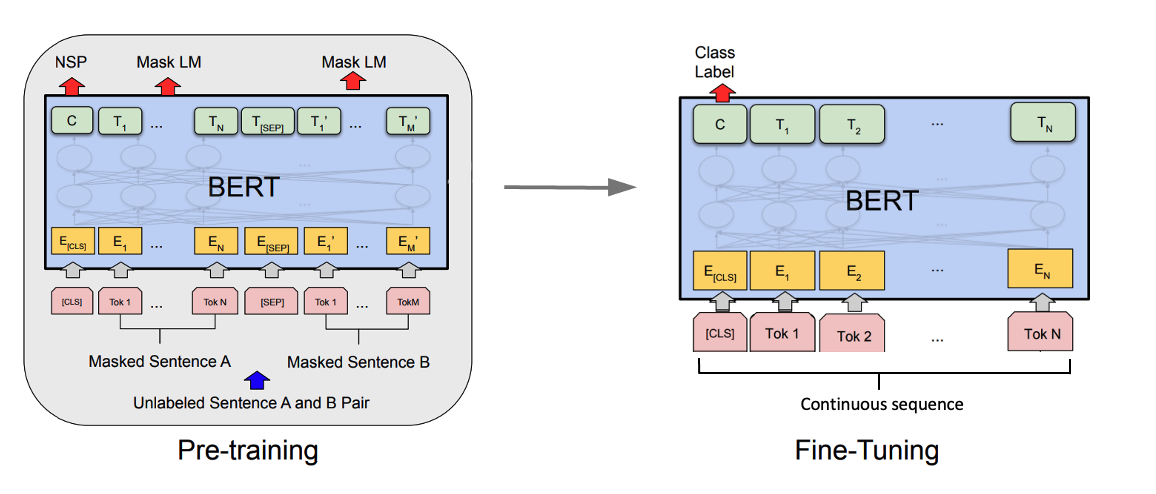
\includegraphics[scale=0.37]{0-img/bert-pretraining-finetuning.png}
    \caption{BERT pre-training and fine-tuning stages, in this case for sequence classification (edited from \cite{bert})}
    \label{fig:bert-pretraining-finetuning}
\end{figure}

Input sequences into BERT must first have special [CLS] and [SEP] tokens added to them. A [CLS] token denotes the beginning of the input sequence, and [SEP] tokens are added between sentences as markers for BERT. The input sequence is then converted to token IDs, segment IDs and attention IDs. For more information on these, see \cite{bert}.

Chun et al. \cite{chun} used BERT to simultanously detect political bias and detect trolls on Twitter, finding that the accuracy, precision and recall of the BERT model far surpassed those of the other models used (SVMs, standard neural networks and convolutional neural networks). They report a highest accuracy of 89\% for the bias detection task. The Bipartisan Press in their analysis \cite{bipartisan-press} found BERT performs much better at predicting both amount of bias and direction of bias than both LSTMs (long short-term memory networks) and ULMFiT (a transfer-learning-based model), as well as an ensemble model built from the two. They obtained even better results when using RoBERTa \cite{roberta}, a version of BERT that has been pre-trained for longer and with more data. Baly et al. \cite{baly-acl2020} used BERT contextualised word embeddings extracted from article text as an input feature to an SVM trained to detect bias. They report a highest F1 of 81.27\% and accuracy of 81.83\%, both much higher than for their earlier SVM classifier without BERT.

\section{Reddit} \label{sec:reddit}

Reddit is one of the most popular social media platforms today, with over 430 million active users as of April 2020 \cite{sattelberg}. Reddit is characterised by its unique `subreddits' feature: communities that any user can join in order to read posts, comment, and post themselves about a particular topic. Subreddits begin with `r/' followed by the topic name, for example popular subreddits include r/sports, r/astronomy, r/books and r/cooking. More politically-oriented subreddits include r/liberal, r/conservative, r/worldpolitics, r/ukpolitics, and many more. Reddit users can `upvote' or `downvote' any posts or comments, which increases/decreases their visibility to other users.

\begin{figure}
    \centering
    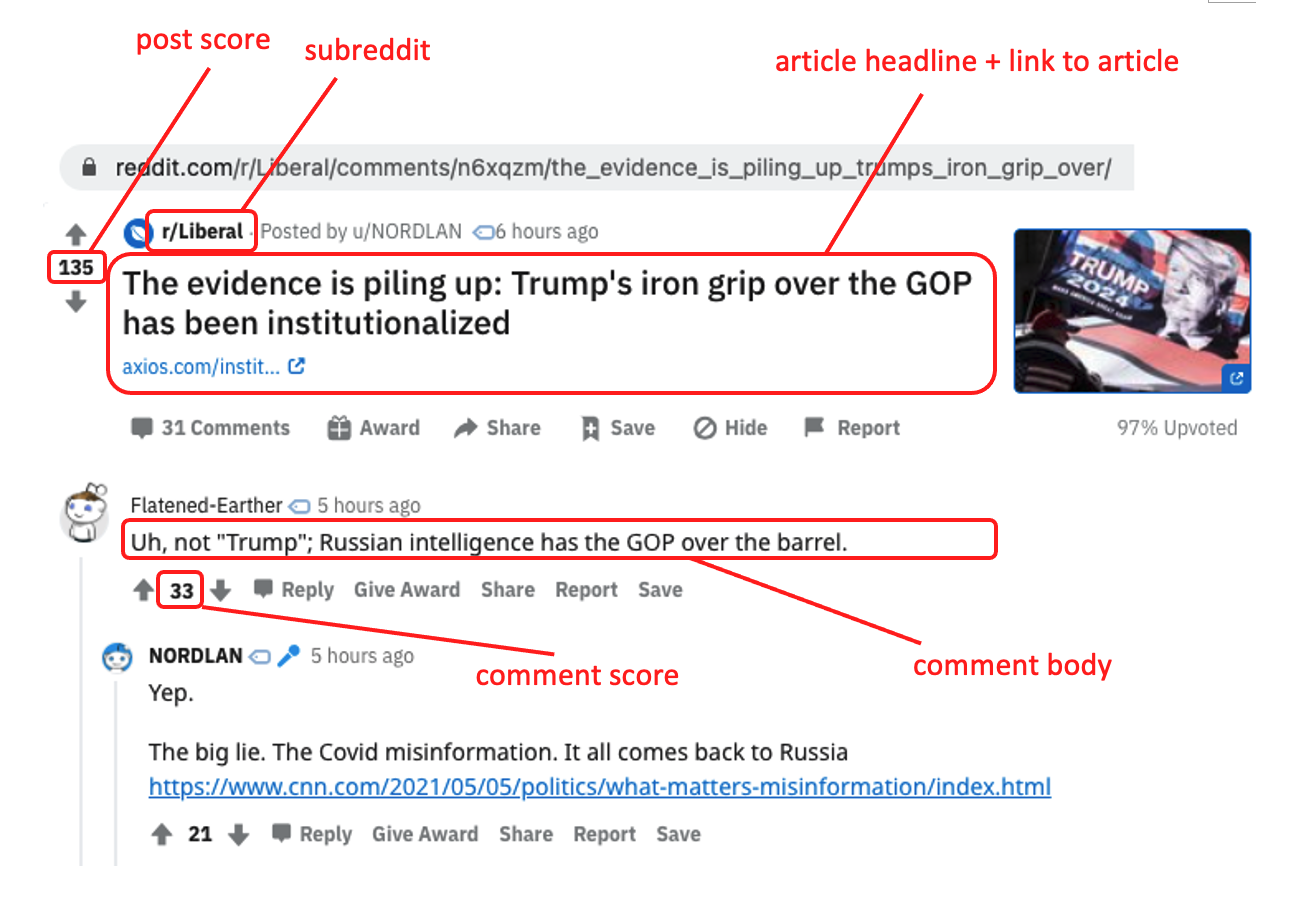
\includegraphics[scale=0.27]{0-img/annotated-reddit-post.png}
    \caption{The anatomy of a typical Reddit post}
    \label{fig:annotated-reddit-post}
\end{figure}

Figure \ref{fig:annotated-reddit-post} shows what a typical Reddit post looks like. The post and comment `scores' are simply the sum of any upvotes and downvotes that particular post or comment has - an upvote counts as +1, a downvote as -1. Reddit provides a `top posts' feature for each subreddit that allows users to search for the top posts by score in the last day/week/month/year.

A typical post on a political subreddit involves a link to a particular news article, and a comment stream with reactions from people who frequent that subreddit. Most often this will be the users that are actually subscribed to that subreddit, but occasionally there is discourse between subscribers and non-subscribers.

\subsection{Collecting Reddit data} \label{subsec:collecting-reddit-data}

Reddit data can be collected from the public Reddit API \cite{reddit-api}, or from online data dumps of Reddit posts such as the PushShift dataset \cite{pushshift}.

The Reddit API yields JSON files that describe any given subreddit, post, comment or user on the website. Examples of information exposed by the API include subreddit names, descriptions, post content, links to webpages referenced in posts, post scores, comment text and comment scores. The API also provides features to search for the most recent posts in a particular subreddit, and the top $ n $ posts in that subreddit in the last day/week/month/year. The API is most commonly accessed with the Python \texttt{praw} package \cite{praw}.

The PushShift dataset is a large data dump of Reddit posts, comments, subreddit information and more, assembled by Reddit user Jason Baumgartner. It is available online at \url{https://files.pushshift.io/reddit/} \cite{pushshift}. The dataset contains Reddit posts and Reddit comments arranged by month from June 2005 (the month Reddit was created) through to December 2019 - in total the dataset contains around 651 million posts and 5.6 billion comments. The dataset contains almost all the same information the Reddit API exposes, however one cannot fetch the top $ n $ posts in that subreddit at a particular point in time.

In terms of data annotated by political bias, there is a severe lack of published datasets of Reddit content in this format. Most papers exploring political bias on Reddit (see Section \ref{subsec:readership-bias-social-media}) do not make their data available publicly.

\section{Readership bias} \label{sec:readership-bias}

We define readership bias as the bias shown by audiences, rather than by a news source. A significant portion of readership bias research so far has focused on analysing the sentiment of readers - early work on this was done by Lin et al. \cite{lin}, who classified news articles by 8 different possible emotions expressed by the reader, recorded as reactions on Yahoo's website. Psychologist Paul Ekman popularised the existence of 6 basic emotions \cite{ekman}: happiness, sadness, anger, fear, disgust and surprise. Strapparava et al. \cite{strapparava} used this emotion model to detect sentiment analysis in news headlines with a Naive Bayes classifier. Tan \cite{chien-tan} also created a readership bias model based on the 6 emotions, and separately created a model to predict the distribution of Facebook Reactions on posts containing links to news articles.

Baly et al. \cite{baly-acl2020} interestingly used features taken from readers' online profiles as a predictor for a news source's political bias. Baly's model of thinking was that a source's audience characterises how biased that source is and in what direction (that is, readership bias determines bias in the source). This differs from our line of thinking, which is that bias in the source determines readership bias. It is hard to say which of these philosophies is `correct' - indeed there may be an element of both at play, that is news organisations will decide what to publish based on their target audience, and at the same time their target audience will change depending on what they publish.

\subsection{Detecting readership bias on social media} \label{subsec:readership-bias-social-media}

Social media is increasingly becoming a hub for political discussion and discourse. Garimella \& Weber \cite{garimella} analysed the political polarisation of Twitter discussions over time using retweets and hashtags used by 670,000 Twitter users, finding that polarisation increased by around 10-20\% between 2009 and 2016. Rao et al. \cite{rao} used SVMs trained on n-gram features extracted from tweet text to predict the political affiliation of various Twitter users. Voong et al. \cite{voong} compared Naive Bayes classifiers, SVMs, logistic regression, and random forests with gradient boosting in predicting political polarity of tweets, also using an n-gram approach, finding logistic regression and random forests to give the highest accuracy and F1 scores, and Naive Bayes to give the worst.

Other social media platforms such as Reddit have been less explored. Kane \& Luo \cite{kane} carried out an exploration into political communities on Reddit, examining whether non-political subreddits still exhibit some unconscious political leaning. They did this by analysing comments across different posts within these subreddits and using Latent Dirichlet Allocation (LDA) to see which topics appear most frequently in each subreddit. This topic model was then used to train a classifier to predict the political bias of a subreddit, based on its most-common topics. They were able to achieve a highest accuracy of 85.2\% with an SVM classifier using n-gram features. Since LDA is an unsupervised method, Kane \& Luo didn't have to source any Reddit data annotated by political bias, which is extremely scarce.

Predicting support for specific political figures on social media is a popular task, especially during widely-publicised elections such as the 2016 and 2020 US elections. Massachs et al. \cite{massachs} predict support for Donald Trump using a combination of homophily and social feedback exhibited on r/The\_Donald, a popular subreddit centred around support for Donald Trump. They report a highest accuracy of 35.5\%, suggesting this problem is significantly more challenging than simply detecting left/right-wing bias. It is worth noting that the authors use participation in r/The\_Donald to annotate Reddit users as Trump supporters or not, suggesting they assume only Donald Trump supporters will post in r/The\_Donald. We examine this assumption in Chapter \ref{chap:reddit-data}.

\section{Transfer learning} \label{sec:transfer-learning}

Transfer learning is the study of training a machine learning model for a particular problem A, and applying the model to a different but related problem B. Transfer learning may be explored when it is hard obtaining suitable annotated training data for problem B, or because training for problem B would take too long otherwise.

One popular example of transfer learning is in BERT models - BERT is pre-trained on text from BookCorpus and English Wikipedia \cite{bert} for the tasks of masked language modelling and next sentence prediction, and is later fine-tuned for the target task at hand (which could be sentence classification, question answering, named entity recognition, etc.). Another popular form of transfer learning occurs in imaging problems, where CNNs pre-trained for image classification on ImageNet are then fine-tuned for other tasks such as object detection, image segmentation, or perhaps for further image classification.

In the following, we use notation similar to previous literature \cite{ruder} \cite{pan-survey} to formalise the theory of transfer learning:

A data domain $ \mathcal{D} $ can be formulated as a feature space $ \mathcal{X} $ accompanied by a probability distribution $ P(X) $ over the feature space. Intuitively, a domain is a set of data that exhibits a unique set of characteristics with respect to some feature space. In the real world, different textual domains include literary writing, scientific writing, news article text, tweets, etc. These will all exhibit a different distribution of features if we use a feature space of, say, $n$-dimensional word embeddings.

Given some domain $ \mathcal{D} = (\mathcal{X}, P(X)) $, a task $ \mathcal{T} $ is defined as a set of labels $ \mathcal{Y} $ and a prior (or `ground truth') label distribution $ P(Y) $. A classifier aims to learn the conditional probability distribution $ P(Y | X) $ from some training data $ \{x_i, y_i\}_{i=1}^{n} $.

Given a \textbf{source domain} $ \mathcal{D}_S $ and \textbf{source task} $ \mathcal{T}_S $, along with \textbf{target domain} $ \mathcal{D}_T $ and \textbf{target task} $ \mathcal{T}_T $, the goal of transfer learning is to learn the conditional distribution $ P_T (Y_T | X_T) $ in domain $ \mathcal{D}_T $.

\textit{Transductive transfer learning} is when the target task is the same as the source task (i.e. $ \mathcal{T}_S = \mathcal{T}_T $), however the source domain and target domain may vary, or labelled data may only be available in the source domain. Examples of transductive transfer learning include domain adaptation and cross-lingual learning. \textit{Inductive transfer learning} is when the two tasks are not the same, and labelled data for the target domain is often present. Examples of inductive transfer learning include multi-task learning and sequential transfer learning. 

\subsection{Domain adaptation} \label{subsec:domain-adaptation}

Domain adaptation (also known as cross-domain learning) is a specific case of transductive transfer learning. In this case the source task and target task are identical, however the source and target domains may be different, or labelled target data may not be available (in which case we perform \textit{unsupervised} domain adaptation). Figure \ref{fig:domain-adaptation} shows a typical domain adaptation problem.

\begin{figure}[ht]
    \centering
    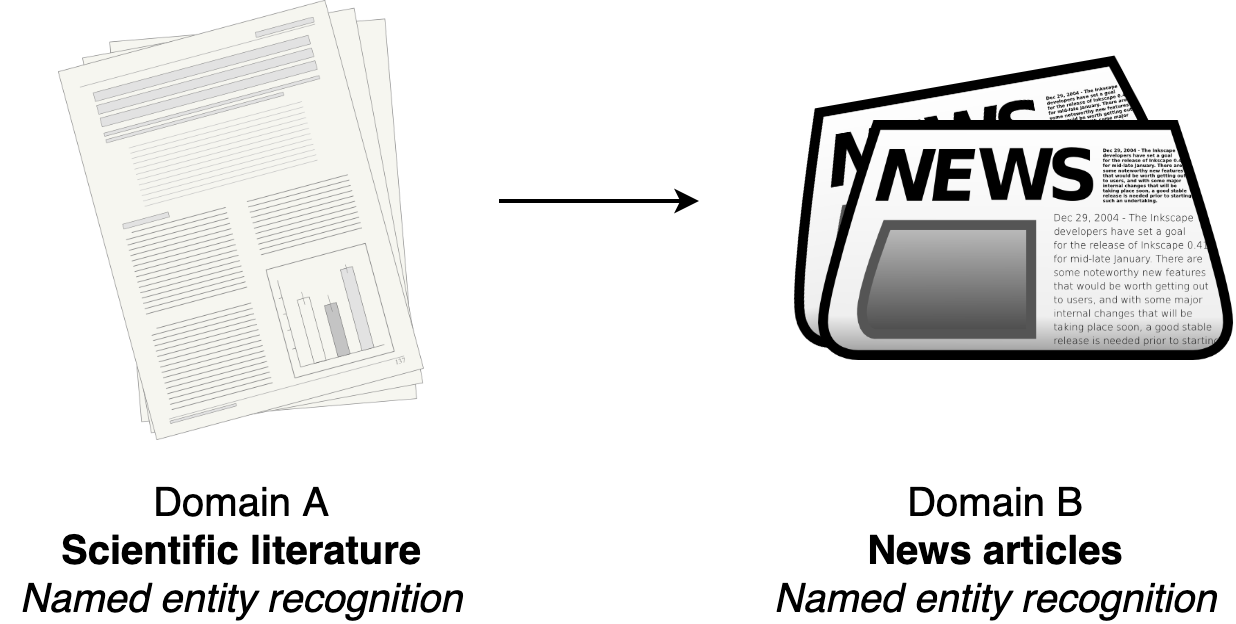
\includegraphics[scale=0.24]{0-img/domain-adaptation.png}
    \caption{An example domain adaptation problem, transferring knowledge from the domain of scientific literature to the domain of news articles, for the task of named entity recognition. Images sourced from Clker \cite{clker}.}
    \label{fig:domain-adaptation}
\end{figure}

\todo{emphasis on unsupervised}

Daumé \& Marcu \cite{daume} initially proposed the idea of `in-domain' and `out-of-domain' data, and applied these ideas to statistical learning theory. Other early work by Blitzer et al. \cite{scl} introduced the idea of structural correspondence learning, where ``pivot features'' are selected that occur frequently in both the source and target domain, and behave similarly in both. This correspondence can then help a classifier perform a task such as POS tagging on the target domain.

Pan et al. \cite{pan-sfa} proposed a spectral feature alignment algorithm that can group domain-specific words into clusters, based on the distances between the domain-independent words in the corpus. Domains-specific words are those that occur most frequently in one domain, whereas domain-independent words occur frequently in both domains. Michelbacher et al. \cite{feature-adaptation} consider domain-\{specific/independent\} features as a whole, and propose the idea of unsupervised feature adaptation for situations where no labelled target domain data is available. A classifier is trained on source domain data, and any domain-independent features are recomputed in an unsupervised fashion to align themselves with the target domain data, before being passed to the classifier to infer on the target domain data. Any domain-specific features are ignored.

The above methods all rely on some manual selection of features that are ``domain independent'' i.e. occur similarly in both the source and target domain. However, recent work has aimed to remove this manual step in the transfer learning process. Myagmar et al. \cite{cdsc} explored using BERT for cross-domain sentiment classification, finding that fine-tuning BERT on the source domain and running inference on the target domain (a process known as \textit{direct transfer}) beat several pre-existing benchmarks for the task, using significantly less training data and with much faster training times in addition.

Further work has been done to extend BERT for domain adaptation. Ye et al. \cite{bert-feature-adaptation} use BERT's layer weights as features in a form of feature adaptation, and Du et al. \cite{domain-aware-bert} explore adding a post-training domain-distinguishing task to BERT's fine-tuning stages, and injecting adversarial learning into BERT.

Han \& Eisenstein propose AdaptaBERT \cite{adaptabert}, a novel unsupervised domain adaptation approach which adds an extra stage of masked language modelling on the target domain during fine-tuning. This gives a significant performance boost to the classifier, especially on words and phrases seen at inference time that were not seen in the source domain at training time (`out-of-vocabulary' terms). AdaptaBERT yields several percentage points higher accuracy than direct transfer methods for a historical English POS tagging task, with 30\% increase in accuracy on out-of-vocabulary terms. AdaptaBERT also outperforms existing methods on a Wikipedia $ \rightarrow $ Twitter transfer learning task.

Gururangan et al. \cite{dont-stop-pretraining} compared this approach, which they name task-adaptive pre-training, to a general domain-adaptive pre-training approach where MLM is performed on a large amount of generic target-domain text that is not necessarily aimed at the specific task at hand. They find a combination of both methods provides the highest classifier accuracy for transfer learning tasks between news articles, IMDB reviews and biomedical scientific papers.

\section{Going forward}

In this chapter we have defined political bias and looked at previous work in detecting political bias in the news with NLP and machine learning. We have discovered that ensemble classifiers are under-explored for this particular problem, which we examine further in Chapter \ref{chap:ensemble-bert}, where we also directly compare existing methods of detecting bias.

We have also defined the related problem of readership bias and explored prior work in detecting readership bias on social media. In this project we seek to explore how domain adaptation between the domains of news articles and social media comments can be exploited to improve accuracy of political bias detection on social media. We aim to tackle Reddit specifically, however we discovered there is a significant lack of Reddit content labelled by political bias online. To remedy this, we create our own such dataset in Chapter \ref{chap:reddit-data}. We then explore domain adaptation for this problem, specifically looking at AdaptaBERT, in Chapter \ref{chap:domain-adaptation}.
\chapter{Detecting political bias with ensemble classifiers and BERT} \label{chap:ensemble-bert}

In this chapter we survey existing models to detect political bias, using the News-Media-Reliability dataset \cite{news-media-reliability}. Baly et al. already provide an SVM classifier that uses the News-Media-Reliability pre-computed features to detect bias (see Section \ref{subsec:svms}). We compare this to other popular classifiers used in literature, as well as ensemble classifiers that have not been explored previously in detail (Section \ref{sec:nmr-ensemble}). We then assemble our own dataset of raw article text, and explore using features learned automatically from the text with BERT (Section \ref{sec:nmr-bert}).

\section{Using ensemble classifiers} \label{sec:nmr-ensemble}

The pre-computed features in the News-Media-Reliability dataset include feature vectors based off article text, Twitter pages, Wikipedia pages and web traffic (see Section \ref{subsec:news-media-reliability} for more details about the dataset). In an ablation study, Baly et al. found that the features extracted from the actual article content provided the best classifier performance, however the Wikipedia, Twitter and web traffic features were not very useful for predicting bias. This intuitively makes sense, as not much extra information about bias can be derived from the Wikipedia or Twitter content of the news source. We therefore don't consider individual Twitter, Wikipedia and web traffic features in our results - we simply compare the performance using all pre-computed features vs only article text features.

\subsection{Data pre-processing}

The News-Media-Reliability features we use are already provided in numerical vector format, so no additional pre-processing needs to be done here. However, there is significant class imbalance among the 7 labels used in the data.

The original labels are \textit{extreme-left, left, center-left, center, center-right, right} and \textit{extreme-right}. We merge \textit{extreme-left} and \textit{extreme-right} into \textit{left} and \textit{right} respectively, due to \textit{extreme-left} being very small in size. We also remove the \textit{left-center} and \textit{right-center} classes, since \textit{right-center} is small in size, and these are ambiguous transitionary classes that can't necessarily be merged into \textit{center} or \textit{left/right}. Table \ref{tab:nmr-class-balancing} shows the class sizes before and after pre-processing.

\begin{table}[h]
    \begin{center}
        \begin{tabular}{|c|c|c|c|c|c|c|}
            \hline
            extreme-left & left & left-center & center & right-center & right & extreme-right \\
            \hline
            21 & 168 & 209 & 263 & 92 & 157 & 156 \\
            \hline
        \end{tabular}
    \end{center} \vspace{5pt}
    \begin{center}
        \begin{tabular}{|c|c|c|}
            \hline
            left & center & right \\
            \hline
            189 & 263 & 313 \\
            \hline
        \end{tabular}
    \end{center}
    \caption{News-Media-Reliability original classes (top) vs. final classes used (bottom)}
    \label{tab:nmr-class-balancing}
\end{table}

There is still some class imbalance between left and right, however the overall imbalance has been greatly reduced.

\subsection{Evaluation}

We compare six classifiers in total: 3 non-ensemble methods (SVMs, multi-layer perceptrons and decision trees) and 3 ensemble methods (random forests, Adaboost and gradient-boosted forests). Random forests are of course an ensemble of decision trees, and Adaboost and gradient-boosted forests both implement different gradient-boosting algorithms.

For each experiment we use 5-fold cross validation, and within each fold we use an 80:20 train/test split. All classifiers are implemented using the Python \texttt{scikit-learn} package \cite{sklearn}, using the \texttt{GridSearchCV} method for hyperparameter tuning.

Results are shown in Table \ref{tab:nmr-ensemble-results}, given to 2 decimal places. The highest performing classifier for each metric is highlighted in \textbf{bold}. We report macro-averaged F1 score, accuracy, mean absolute error (MAE) and macro-averaged mean absolute error ($ MAE^M $). $ MAE^M $ is a weighted average of errors for each class, where the weights are inversely proportional to the size of each class i.e. smaller classes' errors are upweighted more. This metric is much more robust to class imbalance than MAE.

\begin{table}[h]
    \centering
    \small
    \begin{adjustbox}{width=1.1\textwidth,center}
    \begin{tabular}{|c|c|c|c|c|c|c|c|c|c|}
        \hline
        \textbf{Classifier} & \multicolumn{4}{|c|}{\textbf{All features}} & \multicolumn{4}{|c|}{\textbf{Only text-based features}} \\
         & \textbf{Macro-F1} & \textbf{Acc.} & \textbf{MAE} & $ \textrm{\textbf{MAE}}^M $ & \textbf{Macro-F1} & \textbf{Acc.} & \textbf{MAE} & $ \textrm{\textbf{MAE}}^M $ \\
         \hline
         SVM & \textbf{67.07} & \textbf{68.76} & 0.46 & 0.50 & 64.93 & 66.27 & 0.45 & 0.48  \\
         MLP & 54.90 & 60.26 & 0.56 & 0.66 & 58.17 & 61.57 & 0.52 & 0.59 \\
         Decision tree & 48.28 & 49.80 & 0.67 & 0.70 & 49.03 & 49.80 & 0.70 & 0.71 \\
         \hline
         Random forest & 59.52 & 64.71 & 0.49 & 0.57 & 57.95 & 63.53 & 0.51 & 0.60 \\
         Adaboost & 59.04 & 62.48 & 0.53 & 0.61 & 59.23 & 61.44 & 0.54 & 0.59 \\
         Grad-boosted forest & 66.17 & 68.10 & \textbf{0.44} & \textbf{0.48} & \textbf{65.85} & \textbf{67.45} & \textbf{0.44} & \textbf{0.48} \\
         \hline
    \end{tabular}
    \end{adjustbox}
    \caption{Bias detection results using pre-computed features across different classifiers}
    \label{tab:nmr-ensemble-results}
\end{table}

We see that using all features, the highest performing classifiers is the SVM, with gradient-boosted forests coming in a close second. Only using the text-based features, gradient-boosted trees perform the best. Hence ensemble classifiers do show a small improvement ($ \approx $ 1\%) over the other, weaker learners for this particular problem.


Baly et al. report an SVM macro-F1 score of 61.31\% and accuracy of 68.86\%. Our SVM manages to achieve a similar accuracy, however our macro-F1 score is around 6 percentage points higher. This could be attributed to our differences in dealing with class imbalance - Baly et al. merge \textit{center-left} and \textit{center-right} into the \textit{center} class, whereas we actually remove the transitionary classes altogether. Our higher F1 score could signify that keeping a distinct boundary between left-wing and right-wing content improves classifier performance, even if the amount of training data available is reduced. Merging \textit{left-center} and \textit{right-center} into the \textit{center} class may confuse the classifier, causing it to mispredict.

We note for all classifiers except for MLPs, the accuracy and F1-scores are higher using all the features vs only text-based features, however the difference is within around 2 percentage points. This backs up the claims by Baly et al., who report that the non-textual features do not provide much additional information to the model.

The best hyperparameters for our SVM were RBF as the kernel function, degree of polynomial decision boundary = 3, $ C = 100 $ and $ \gamma = 0.001 $. The best gradient-boosted forest hyperparameters were: no. estimators = 100, learning rate = 0.6 and minimum samples in a leaf node = 5.

\section{Using BERT} \label{sec:nmr-bert}

Whereas the previous ensemble classifiers take in manually engineered features, BERT models learn the optimal features straight from the raw text. We therefore create our own dataset of news article text (including headline and article body text). These were scraped from the web using an open source tool called \texttt{NewsScraper} \cite{newsscraper}, which is based off of the Python \texttt{newspaper} \cite{newspaper-python} package.

We scrape from all news sources present in the News-Media-Reliability dataset. After class merging from Section \ref{sec:nmr-ensemble} we have 732 sources to consider. Many of these sources use front-end code formats NewsScraper cannot parse - NewsScraper only managed to scrape articles from 432 of these news sources. We collect a maximum of 5 articles per news source, giving us a total of 1654 news articles (note that not all news sites had 5 available articles to scrape). For each article we store the article headline, article body text, and the political bias label for this news source as given by Media Bias/Fact Check (\textit{left}, \textit{center} or \textit{right}). A portion of the dataset is shown in Figure \ref{fig:nmr-bert-data}. The distribution of classes is shown in Table \ref{tab:nmr-bert-data-classes} - there are a significant amount more right-wing articles than center or left articles.

\begin{table}[h]
    \centering
    \begin{tabular}{|c|c|c|}
        \hline
        left & center & right \\
        \hline
        430 & 567 & 657 \\
        \hline
    \end{tabular}
    \caption{Class distribution in self-assembled article text dataset}
    \label{tab:nmr-bert-data-classes}
\end{table}

\begin{figure}
    \centering
    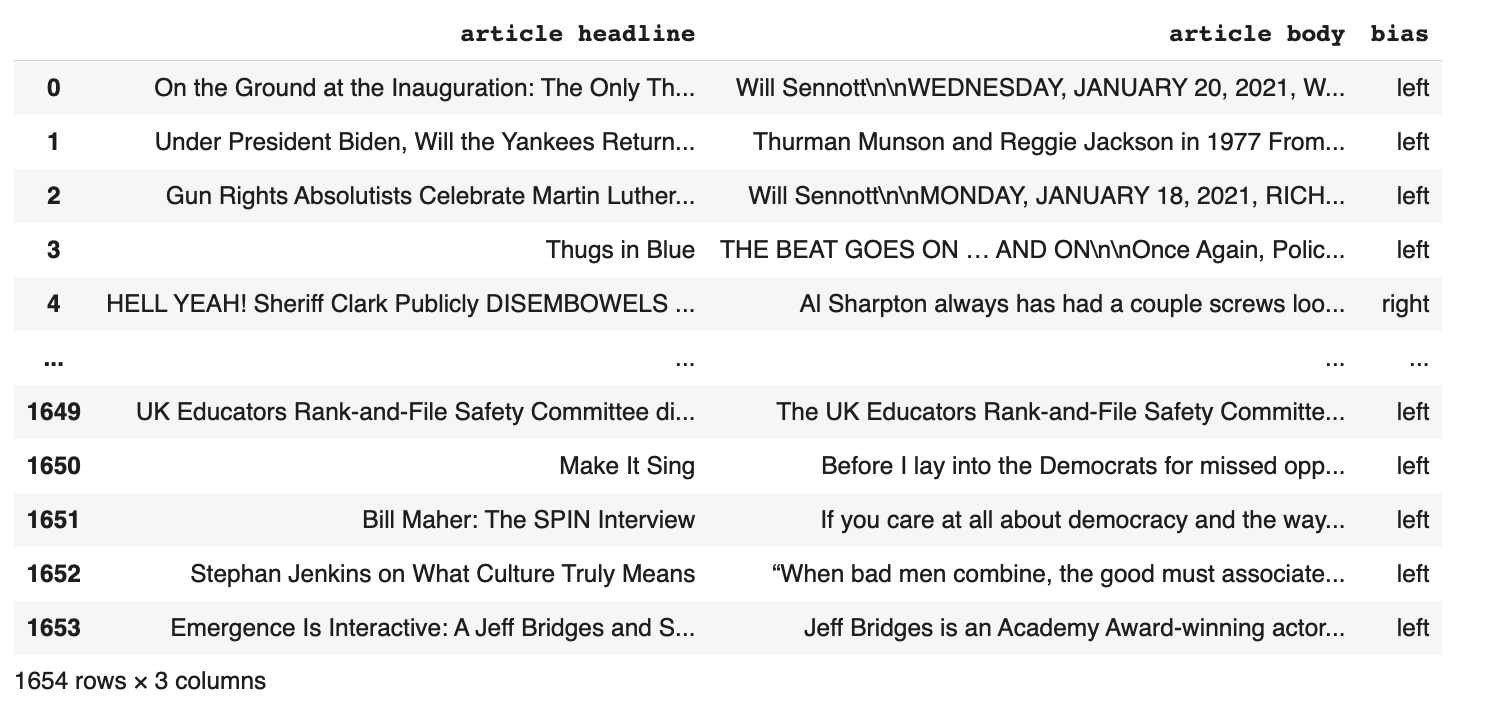
\includegraphics[scale=0.29]{0-img/nmr-bert-data.png}
    \caption{Self-assembled dataset of article headlines, article body text and political affiliation}
    \label{fig:nmr-bert-data}
\end{figure}

\subsection{Data pre-processing}

We pre-process the text by performing lowercasing, punctuation removal, stopword removal and lemmatisation. We opt to keep in exclamation marks and question marks, since BERT can learn features over these to help it detect bias. The Python NLTK \cite{nltk} package is commonly used for stopword removal, however we find it removes words such as `yourselves', `ourselves', `wouldn't', `shouldn't' etc. which could perhaps also be useful for our model. We therefore perform our own more minimalist stopword removal, using mainly basic determiners and prepositions i.e. `I', `you', `in', `at'. Lemmatisation is performed with NLTK's WordNet Lemmatizer \cite{wordnet}.

We encode the labels numerically as \textit{center} := 0, \textit{left} := 1, \textit{right} := 2. We also shuffle the data so that articles from different news sources are spread out in the dataset. The pre-processed dataset is shown in Figure \ref{fig:nmr-bert-data-preprocessed}.

\begin{figure}
    \centering
    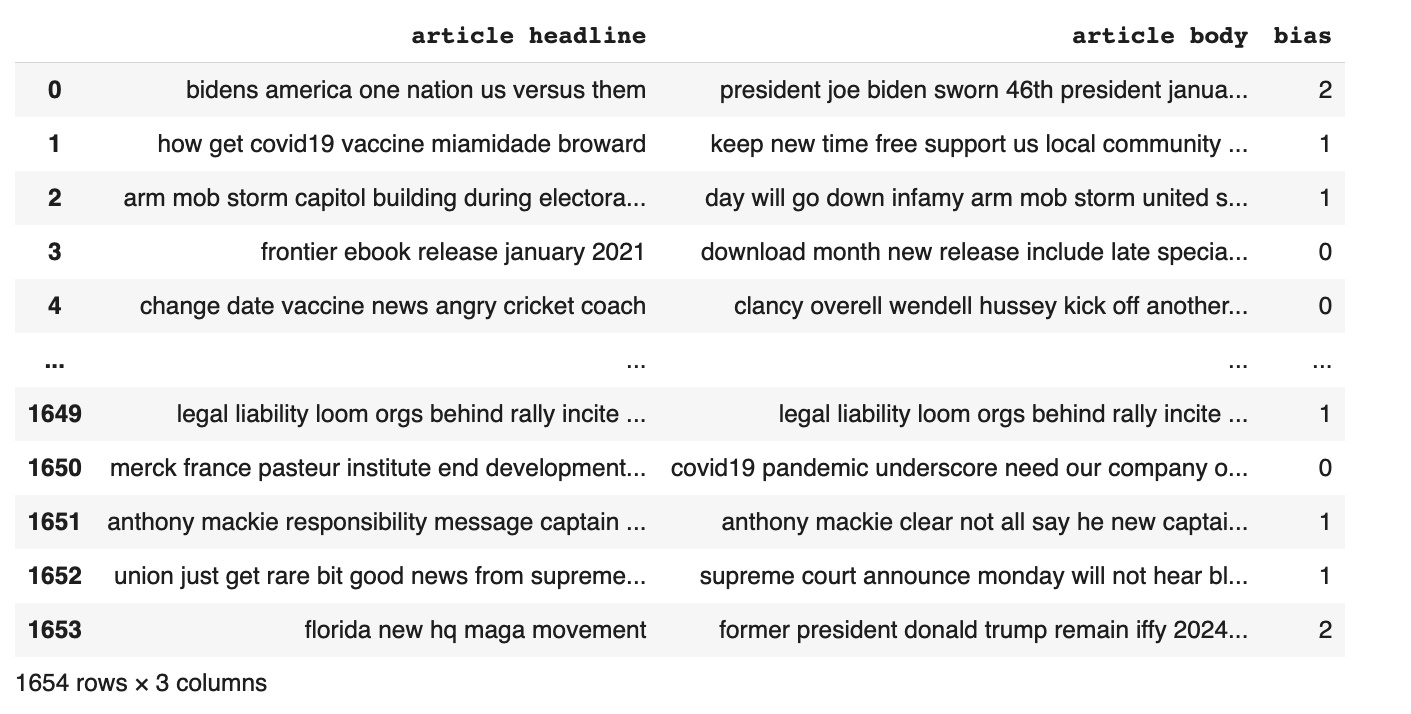
\includegraphics[scale=0.32]{0-img/nmr-bert-data-preprocessed.png}
    \caption{Self-assembled article text dataset after pre-processing}
    \label{fig:nmr-bert-data-preprocessed}
\end{figure}

\subsection{BERT architecture}

Our model is a BERT stack built for sequence classification i.e. with a linear layer at the end and softmax activation to assign a label to the input sequence. We use the pre-trained uncased, base model of BERT since the large model requires too much memory to train with available hardware. We include token IDs, segment IDs and attention masks extracted from the text in our model. A diagram of the model is shown in Figure \ref{fig:bert-sequence-classification}.

BERT only accepts sequences of maximum 512 tokens in length, including the special [CLS] and [SEP] tokens. The maximum headline length with special tokens is 103 tokens, so headlines can be padded up to 512 tokens. However, the maximum article body length is 14,373 tokens, much longer than the limit, so we must truncate article body text to 512 tokens when passing them into BERT.

\subsection{Experimental setup}

We run the BERT sequence classification model using:

\begin{enumerate}
    \item only headlines
    \item only article body text
    \item headlines and body text concatenated together i.e. ``[CLS] \{headline\} [SEP] \{body\}''
\end{enumerate}

Our hypothesis is that using article headlines to predict bias will give higher accuracy than using body text, since headlines distill the essence of the article into just a couple of lines. We also predict using a combined input formed with both headlines and body text will result in higher model accuracy, since more information is being presented to our model.

We use a 70:10:20 train/validation/test split, giving us a training set size of 1157 samples and test set size of 331 samples. We don't use k-fold cross validation with this model due to the small dataset size. With 5 folds each classifier would only be trained with 231 training samples and tested on 66 samples - the training and test sets may not be representative of the overall class distribution.

We use the \texttt{AdamW} \cite{adamw} optimiser, with a learning rate of $ 2 \cdot 10^{-5} $ after hyperparameter tuning. We use a batch size of 10 - we found batches larger than this lead to validation accuracy dropping. We also clip gradient norms to 1 at each training step to prevent any exploding gradients.

\begin{figure}
    \centering
    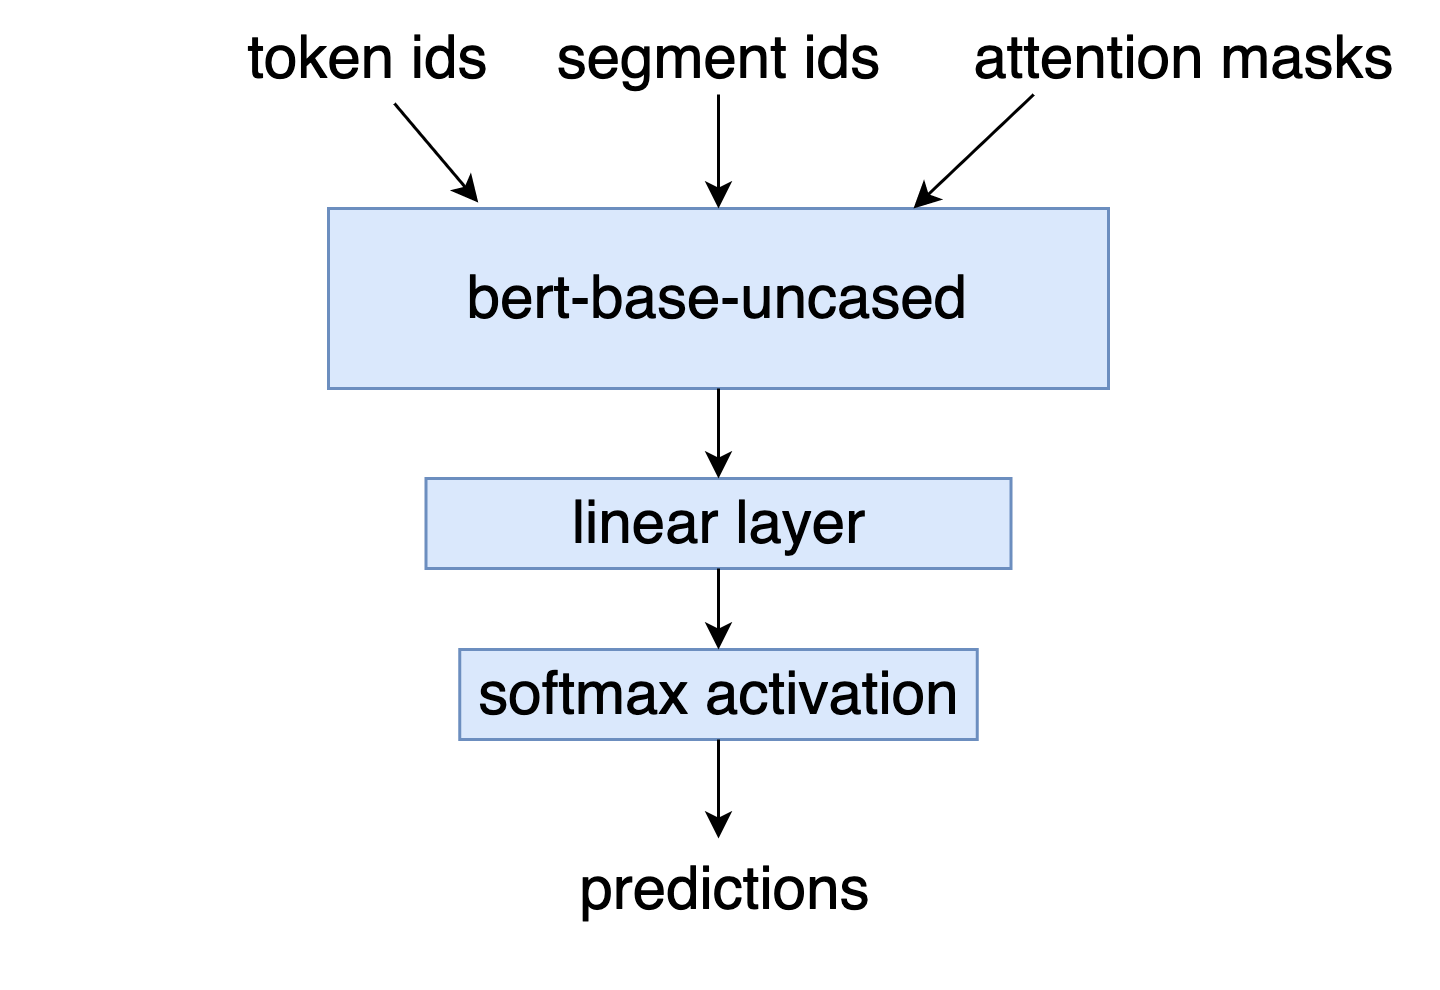
\includegraphics[scale=0.2]{0-img/bert-sequence-classification.png}
    \caption{The BERT sequence classification model}
    \label{fig:bert-sequence-classification}
\end{figure}

\subsection{Evaluation} \label{subsec:nmr-bert-evaluation}

Evaluation metrics comparing the 3 different input types described in the previous section are shown in Figure \ref{fig:nmr-accuracy-f1}.

\todo{compare to earlier classifiers}

\begin{figure}
    \centering
    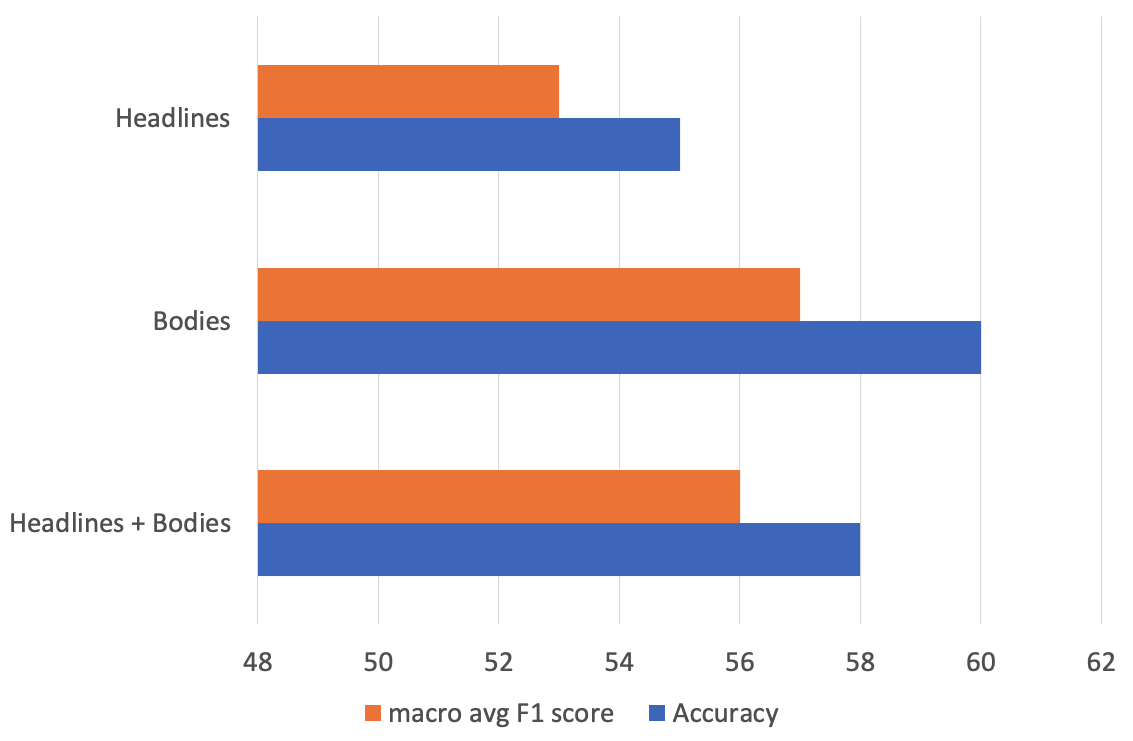
\includegraphics[scale=0.3]{0-img/nmr-accuracy-f1.png}
    \caption{Evaluation metrics for BERT classifier applied to headlines and body text}
    \label{fig:nmr-accuracy-f1}
\end{figure}

We can see using article bodies gives better performance than using article headlines by several percentage points in both accuracy and F1 score, with a highest accuracy of 60\%. Headlines usually distil the content of the article into one or two lines, so this result could be attributed to article bodies simply containing more textual information than headlines (the longest headline in the dataset is only 103 tokens long, much shorter than the maximum 512 tokens allowed).

It's important to note that we have truncated the body text to just the first 512 tokens, and the beginnings of news articles often summarise their main points similar to how a headline would. This could also be why body text gives higher model accuracy than headlines. We explore this further in Section \ref{sec:article-sections} by comparing using the beginning of the article to predict bias vs the middle or the end of the article.

Concatenating headline and body text performs better than simply using headlines, but worse than just using body text. This result is particularly interesting, as our initial hypothesis was that unifying headline and body information would provide the model with more information than using either of the two input types individually. This, however, demonstrates that body text provides more information than any input involving the headlines.

We also explore using RoBERTa for sequence classification, a version of BERT that has been pre-trained further and with more data. Our results are compared in Figure \ref{fig:nmr-roberta-accuracy-f1}. RoBERTa exhibits around the same performance as BERT, with a very minor improvement when using article body text only (61\% accuracy). This demonstrates that further pre-training on the English language does not help the classifier detect bias more easily. 

\begin{figure}
    \centering
    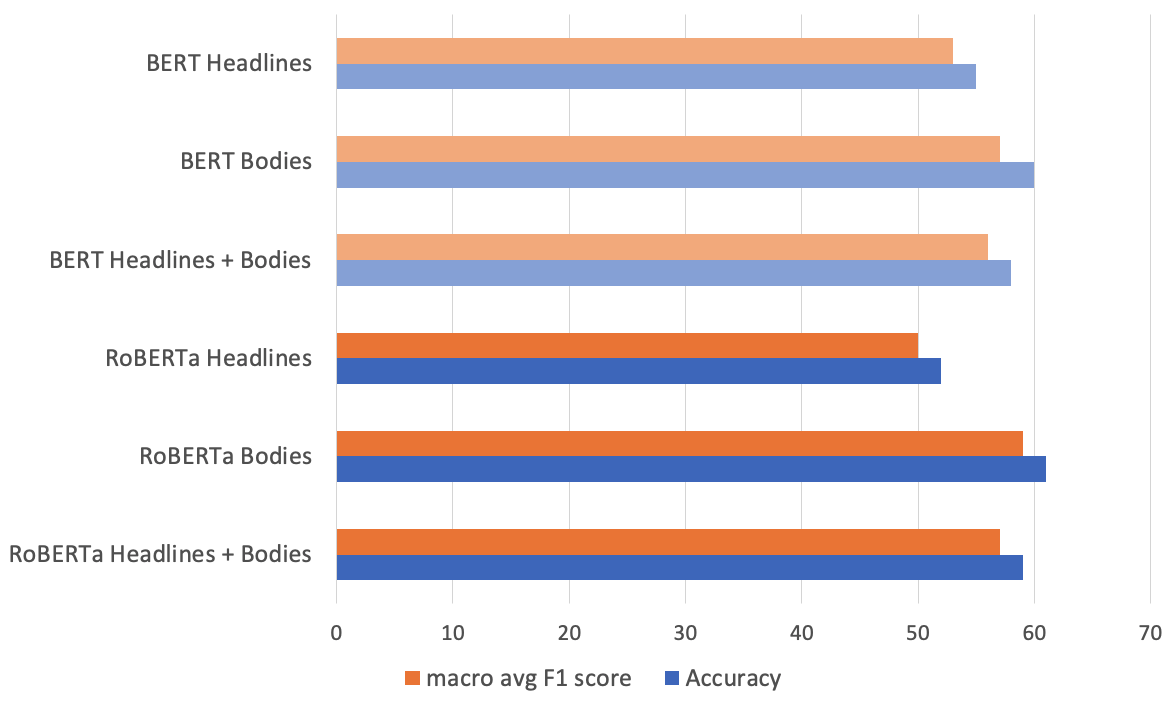
\includegraphics[scale=0.35]{0-img/nmr-roberta-accuracy-f1.png}
    \caption{Evaluation metrics for RoBERTa classifier compared to BERT}
    \label{fig:nmr-roberta-accuracy-f1}
\end{figure}

Chun et al. report an accuracy of 89\% when using BERT to detect political bias in the Russian Troll dataset \cite{russian-troll}, a collection of tweets posted by Russian troll accounts. Our highest accuracy of 61\% is much lower than this. One reason for this discrepancy could be availability of training data - the Russian Troll dataset contains around 3 million tweets, whereas our dataset is very small in comparison, consisting of only 1654 text samples.

Building off the RoBERTa idea, further work could be done examining BERT models pre-trained via predicting bias in text, on top of MLM and NSP, to see if this improves bias detection. We could also explore applying BERT to a much larger dataset - while our self-assembled dataset contains high-quality raw article text, it contains a very small number of text samples compared to other datasets explored in previous literature.

One point to note is that BERT models split tokens up using a subword-level vocabulary, created using the Wordpiece \cite{wordpiece} algorithm. Names therefore get split into subwords after tokenisation, e.g. ``biden'' becomes [`bid', `\#\#en'] and ``covid'' becomes [`co', `\#\#vid']. This could limit the effectiveness of names within the BERT model, since the model will treat the `bid' and `co' tokens just like any other instances of those words in the text. We find that ``biden'' occurs 2,696 times in the dataset, but the `bid' token otherwise only occurs 11 times, so this is not a huge problem in this case. However, ``covid'' occurs 1,201 times in the dataset and the `co' token otherwise occurs another 529 times, which could lead to confusion in the BERT model. Other weaknesses of Wordpiece tokenisation have been explored previously \cite{wordpiece-weaknesses}.

\subsection{Detecting bias from particular article sections} \label{sec:article-sections}

In this section we purely focus on article body text. We want to examine which section of an article (beginning, middle or end) is most helpful to the classifier in determining political bias.

We use the same dataset as in the previous sections. Instead of letting the BERT tokenizer truncate articles to just the first 512 tokens, we isolate 512 tokens from the beginning, middle, and end of article bodies, and pass these into our BERT classification model. Our hypothesis is that using the beginning/end of article text will give higher model accuracy than using text in the middle, since articles often introduce or conclude their main ideas in these sections, and so evidence of political bias will be more evident.

We use the same experimental setup and hyperparameters as in the previous section. Results are shown in Figure \ref{fig:nmr-beginning-middle-end}.

\begin{figure}
    \centering
    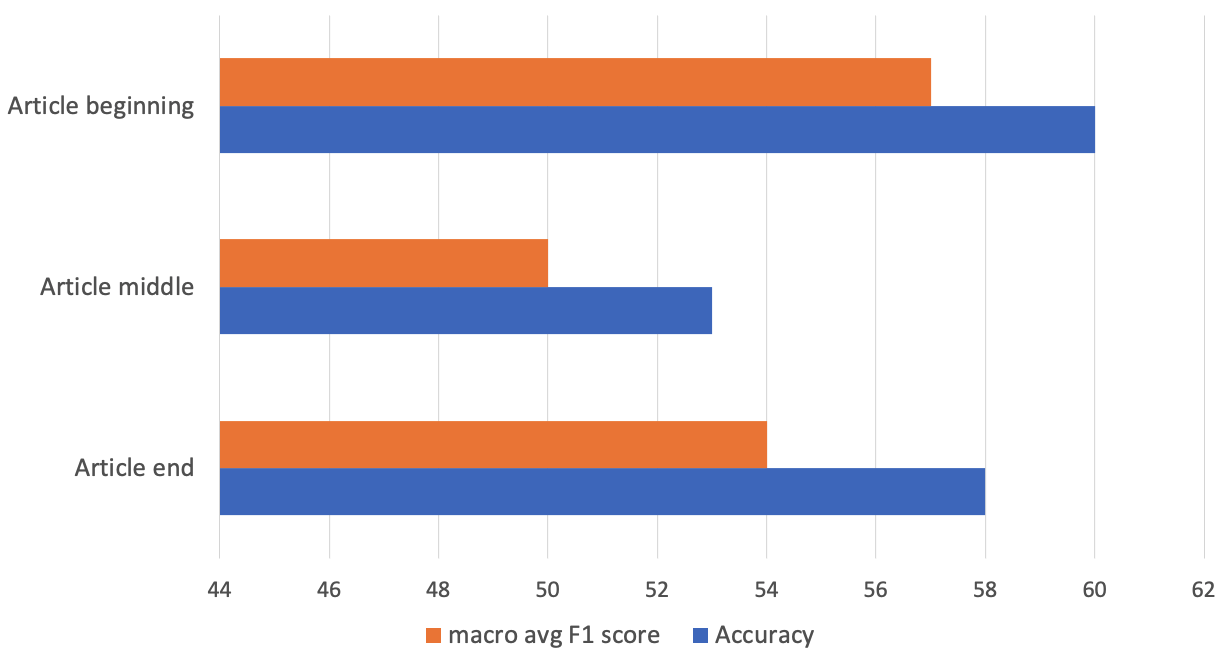
\includegraphics[scale=0.33]{0-img/nmr-beginning-middle-end.png}
    \caption{Evaluation metrics using beginning, middle or end of article text to predict bias}
    \label{fig:nmr-beginning-middle-end}
\end{figure}

We can see our hypothesis has been validated - the model accuracy is better when using text from the beginning or end of an article, rather than from middle sections. Interestingly using introductory text gives a higher accuracy than using concluding text - since introductory text is the first thing the reader sees, perhaps this text is more representative of the overall bias of the article.

The accuracies using the introduction and conclusion of the body text are 60\% and 58\% respectively, however the accuracy we achieved from using article headlines (in the previous section) is 55\%. Therefore, using either the introduction or conclusion of the body text is actually more useful to the classifier than using any headline information at all.
\chapter{Developing a cross-domain Reddit dataset} \label{chap:reddit-data}

In this chapter we discuss the methodology of creating a novel cross-domain dataset containing a set of news articles that have been shared on Reddit, and the accompanying Reddit comments, specifically aimed at machine learning tasks for detecting political bias.

\todo{to fulfil our project objectives of detecting political bias on social media, we need a dataset. none exist in literature}

We create our own dataset of Reddit content annotated by political bias since, as mentioned in Section \ref{subsec:collecting-reddit-data}, no pre-existing datasets of this type exist in the literature. Using a pre-existing dataset would mean we can compare classifier performance to baselines given in previous literature.

On top of this, justifying how our data is collected and how we ensure the data is of high-quality is a fundamental step in the machine learning process that is often ignored - usually a model is only as good as the training data it receives \cite{ilyas}.

The news articles and the comments addressing those articles present different (but related) domains of text that can be explored and compared. We examine similarity between the different domains, as well as the sentiment expressed in our dataset.

\section{Designing a high-quality dataset}

Here we look at several issues faced in creating a high-quality dataset.

\subsection{Finding suitable annotations} \label{subsec:annotations}

One major design decision we face is how to find suitable annotations, since this influences later decisions on where (and how) to source our data.

Typically, posts and comments on social media are not annotated with political leaning, perhaps explaining why the task of exploring political bias on this medium is such a challenging one. However, we can exploit one of the unique features of Reddit, that of subreddits. Posts and comments on Reddit are naturally grouped into communities, and a wide range of popular and politically-related subreddits are available to browse on Reddit, such as r/liberal, r/conservative, r/republican, etc. These subreddit titles provide natural political-bias annotations for the content displayed within each of those subreddits.

One key assumption to examine here is that all content under a particular subreddit will necessarily follow that particular political leaning. For example, whereas most comments in r/liberal may be from subscribers to that subreddit, nothing stops members of another subreddit such as r/conservative from leaving comments under r/liberal and starting a discussion.

However, it has been shown that this occurs very infrequently. A study by Guimaraes et al. \cite{guimaraes} quantified and examined cases of \textit{harmony} and \textit{dispute} among Reddit posts, where \textit{dispute} is defined as a comment thread where one particular set of comments attracts a notable amount of downvotes from the community, and \textit{harmony} is a comment thread where no such set of downvoted comments exists. They find that in two major political subreddits (r/politics and r/worldpolitics) harmonious discourse makes up the majority of all comments, and disputes only occur in around 2\% of comments. This reinforces the assumption we make that content within a particular subreddit will most likely follow that political leaning, since political conversations or arguments between users with opposing viewpoints will almost always contribute to dispute.

In cases where harmonious discourse may not make up a significant portion of all comments, we protect against this by selecting only posts and comments with high upvote counts. Content with more upvotes are more likely to follow the overall bias leaning of the subreddit, so selecting these will almost guarantee the subreddit-name annotations apply to that text. The selection process we use is shown in Algorithm \ref{alg:reddit-data-collection}.

\begin{algorithm}
	\caption{Reddit dataset collection} \label{alg:reddit-data-collection}
	\begin{algorithmic}[1]
	    \State \textit{subreddit list} = [...] \Comment{See Section \ref{subsec:selecting-subreddits}}
		\For {\textit{subreddit} in \textit{subreddit list}}
		    \State Assign \textit{subreddit} a bias label
		    \State Get top 300 \textit{posts} this year with score > 10
		    \For {\textit{post} in \textit{posts}}
		        \State Store linked article (headline + article body)
		        \State Get all \textit{comments} with score > 10
		        \For {\textit{comment} in \textit{comments}}
		            \State Store comment text
		        \EndFor
			\EndFor
		\EndFor
	\end{algorithmic} 
\end{algorithm}

\subsection{Selecting subreddits} \label{subsec:selecting-subreddits}

Since our annotating process relies on subreddit titles, we must select subreddits that explicitly have a political leaning in their name. Examples include r/liberal, r/democrats, etc.

Our original plan was to keep the 3 labels used for our methods in Chapter \ref{chap:ensemble-bert}: \textit{left}, \textit{center} and \textit{right}. However, it is quite hard to identify accurate ``centrist'' subreddits, due to the vague definition of centrism. Furthermore, subreddits that by name may appear to be fairly centrist e.g. r/worldpolitics or r/politicaldiscussion, have been shown to be left-leaning due to Reddit's overall left-leaning bias \cite{tyler}. We therefore restrict our classification problem to only 2 labels: \textit{left} and \textit{right}.

One simple way of collecting verifiably left/right-wing content is to explore subreddits that follow politicians themselves, e.g. r/obama. We look at collecting data from subreddits that follow recent US presidential election candidates, such as Barack Obama and Hillary Clinton. However, one problem is that many of the subreddits related to the 2016 and 2020 Republican Party candidate, Donald Trump, have been banned permanently from Reddit (such as r/The\_Donald). We mitigate this issue by selecting content from r/sh*tliberalssay, a popular right-wing subreddit that has attracted many Trump supporters in recent years. The subreddit focuses on archiving ``the worst liberals on Reddit'' according to the subreddit description, which may prove to be an issue if the posts in the subreddit link to left-wing news articles, however the vast majority of link posts are actually links to images, and so don't get picked up by our scraper.

The full list of subreddits we collect data from is shown in Table \ref{tab:subreddit-list}.

\begin{table}[ht]
    \centering
    \begin{tabular}{|c|c|}
        \hline
        \textbf{Subreddit} & \textbf{Bias Label} \\
        \hline
        r/liberal & left \\
        r/conservative & right \\
        r/democrats & left \\
        r/republican & right \\
        r/obama & left \\
        r/hillaryclinton & left \\
        r/sandersforpresident & left \\
        r/sh*tliberalssay & right \\
        r/libertarian & right \\
        \hline
    \end{tabular}
    \caption{Scraped subreddits and their assigned bias annotations}
    \label{tab:subreddit-list}
\end{table}

\subsection{Resolving class imbalance}

One step we perform to improve the reliability of this dataset is to balance the \textit{left} and \textit{right} classes. Our dataset before balancing contains 992 Reddit posts (i.e. 992 news articles, since the posts are simply links to articles) and 50,608 comments. The class distributions in both articles and comments are shown in Table \ref{tab:reddit-classes-before-balancing}. We see that the majority class present in articles is \textit{left}, but the majority class in comments is \textit{right}, presenting a challenge as to how to resolve class imbalance overall.

\begin{table}[ht]
    \begin{center}
        \begin{tabular}{|c|c|}
            \hline
            left & right \\
            \hline
            600 & 392 \\
            \hline
        \end{tabular}
    \end{center} \vspace{5pt}
    \begin{center}
        \begin{tabular}{|c|c|}
            \hline
            left & right \\
            \hline
            5,977 & 44,631 \\
            \hline
        \end{tabular}
    \end{center}
    \caption{Class distributions in news articles (top) and Reddit comments (bottom) before balancing}
    \label{tab:reddit-classes-before-balancing}
\end{table}

We can't resolve class imbalance in articles and comments independently, since we need to preserve data integrity by only keeping comments for which the articles they are addressing are still present in the dataset, and vice versa. We must therefore balance either articles or comments, and then propagate changes through to the other domain by adding/deleting invalidated data. Thus we can only perfectly balance either articles or comments - the other domain will remain somewhat unbalanced in either case.

We first try balancing articles by downsampling the minority class and then removing all comments that correspond to deleted submissions. However, this leads to catastrophic class imbalance in comments (\textasciitilde 44,000 \textit{right} comments vs \textasciitilde 2000 \textit{left} comments). We therefore balance comments first through downsampling and then propagate changes to the articles - this leads to a much more manageable class imbalance in articles. The final class distributions are shown in Table \ref{tab:reddit-classes-after-balancing}.

\begin{table}[ht]
    \begin{center}
        \begin{tabular}{|c|c|}
            \hline
            left & right \\
            \hline
            419 & 387 \\
            \hline
        \end{tabular}
    \end{center} \vspace{5pt}
    \begin{center}
        \begin{tabular}{|c|c|}
            \hline
            left & right \\
            \hline
            5,977 & 5,977 \\
            \hline
        \end{tabular}
    \end{center}
    \caption{Class distributions in news articles (top) and Reddit comments (bottom) after balancing}
    \label{tab:reddit-classes-after-balancing}
\end{table}

Our final dataset therefore has 806 articles and 11,954 comments. This is a dramatic reduction in the number of comments, but is necessary to balance classes without upsampling.

The distribution of subreddits in our dataset is shown in Table \ref{tab:subreddit-distribution}.

\begin{table}[ht]
    \centering
    \begin{tabular}{|c|c|c|c|}
        \hline
        \textbf{Bias Label} & \textbf{Subreddit} & \textbf{No. Articles} & \textbf{No. Comments} \\
        \hline
        \multirow{5}{2em}{left} & r/liberal & 255 & 2,332 \\
        & r/democrats & 27 & 646 \\
        & r/obama & 33 & 42 \\
        & r/hillaryclinton & 59 & 192 \\
        & r/sandersforpresident & 45 & 2,765 \\
        \hline
        \multirow{4}{2em}{right} & r/conservative & 157 & 3,202 \\
        & r/republican & 37 & 155 \\
        & r/sh*tliberalssay & 4 & 53 \\
        & r/libertarian & 189 & 2,567 \\
        \hline
        \multicolumn{2}{c|}{} & \textbf{806} & \textbf{11,954} \\
        \cline{3-4}
    \end{tabular}
    \caption{Subreddit distribution in our dataset}
    \label{tab:subreddit-distribution}
\end{table}

We can see most articles are sourced from r/liberal, r/conservative and r/libertarian. Furthermore, most comments from r/liberal, r/sandersforpresident, r/conservative and r/libertarian.

\subsection{Avoiding concept drift}

Since we are storing cross-domain data for the purpose of comparing between textual domains, we must make sure to keep all other possible variables constant across all our data (e.g. time, geography), so we don't inadvertently introduce other relationships into our data. This is known as ``concept drift'' \cite{concept-drift}.

We keep time domain the same across all data by only selecting posts from the current year (see Algorithm \ref{alg:reddit-data-collection}). We also keep geographical domain the same across all content by selecting only from mainly US-based subreddits (see Table \ref{tab:subreddit-list}). In fact this restriction does not matter too much, since over 70\% of Reddit users are based in the US anyway \cite{sattelberg}.

\section{Data sources}

In collecting data from Reddit there are two main available sources we consider - the public Reddit API, or the PushShift Reddit dataset (see Section \ref{subsec:collecting-reddit-data}).

The benefits of using the PushShift dataset are that billions of posts and comments have already been scraped from Reddit, so less time and work is needed to manually scrape Reddit. The data is wide-ranging and covers thousands of subreddits, including the subreddits we selected in Section \ref{subsec:selecting-subreddits}. However, Gaffney \& Matias \cite{pushshift-problems} have discovered several major warning signs about the PushShift dataset, most notably concerning large amounts of missing subreddit data, and corrupted data that doesn't make any sense (e.g. comments with timestamps earlier than the post itself).

On top of this, the main benefit of the Reddit API is that the top $ n $ posts of the last week/month/year can be collected, which is not provided in the PushShift data. This is ideal for our collection strategy as discussed in Section \ref{subsec:annotations}, since we want to collect posts and comments that have collected the most upvotes possible, which are grouped in the `top' category as provided by Reddit. We therefore scrape all our data using the Reddit API.

\section{Examining similarity between domains} \label{sec:domain-similarity}

In order to assess the viability of domain adaptation between the domains in our dataset, we look at the similarity between the domains. We model our dataset as containing 3 textual domains - article headlines, article body text, and Reddit comment text.

We compare the Jaccard distance between vocabularies in each domain, which will show us how many words are shared between the domains. For any two sets of words $ A $ and $ B $, the Jaccard distance between them is formulated as:

\begin{equation}
    J(A, B) = \frac{|A \cap B|}{|A \cup B|}
\end{equation}

i.e. the number of words shared divided by the total number of words in both sets. Thus, for all $ A $ and $ B $,  $ 0 \leq J(A, B) \leq 1 $, where 0 indicates zero similarity and 1 indicates perfect similarity (i.e. the sets are identical).

The Jaccard distances between each possible pairing of domains are shown in Table \ref{tab:jaccard-distances}, to 3 s.f. We can see that the similarity between headlines and both other domains is very low. This is surprising - we would expect headlines and bodies to share a similar vocabulary since any article headline will have been derived from its corresponding body text, from the same author and for the same news source, and so we would expect language used to be similar. However, there is a significant similarity between article body text and Reddit comments, suggesting these domains are good candidates for domain adaptation. This is explored further in Chapter \ref{chap:domain-adaptation}.

\begin{table}[ht]
    \centering
    \begin{tabular}{|c|c|}
        \hline
        \textbf{Domain Pairing} & \textbf{Jaccard Distance} \\
        \hline
        article headlines - article bodies & 0.0303 \\
        article headlines - comments & 0.0352 \\
        article bodies - comments & 0.443 \\
        \hline
    \end{tabular}
    \caption{Jaccard distances between domains in our dataset}
    \label{tab:jaccard-distances}
\end{table}

A Venn diagram showing overlap between vocabularies of the 3 domains is shown in Figure \ref{fig:vocab-venn-diagram}, with the size of each set depicted. We can see a large overlap of 159,472 words between article body and comment vocabularies, thus the high Jaccard distance between these 2 domains. However, there are still a large number of words in the article body and comment vocabularies that don't overlap with any other vocabularies (130,123 and 80,594 respectively). Almost all words in article headlines also appear in both article bodies and article comments, however the large sizes of the latter two domain vocabularies leads to the very low Jaccard distance between headlines and these domains.

\begin{figure}[ht]
    \centering
    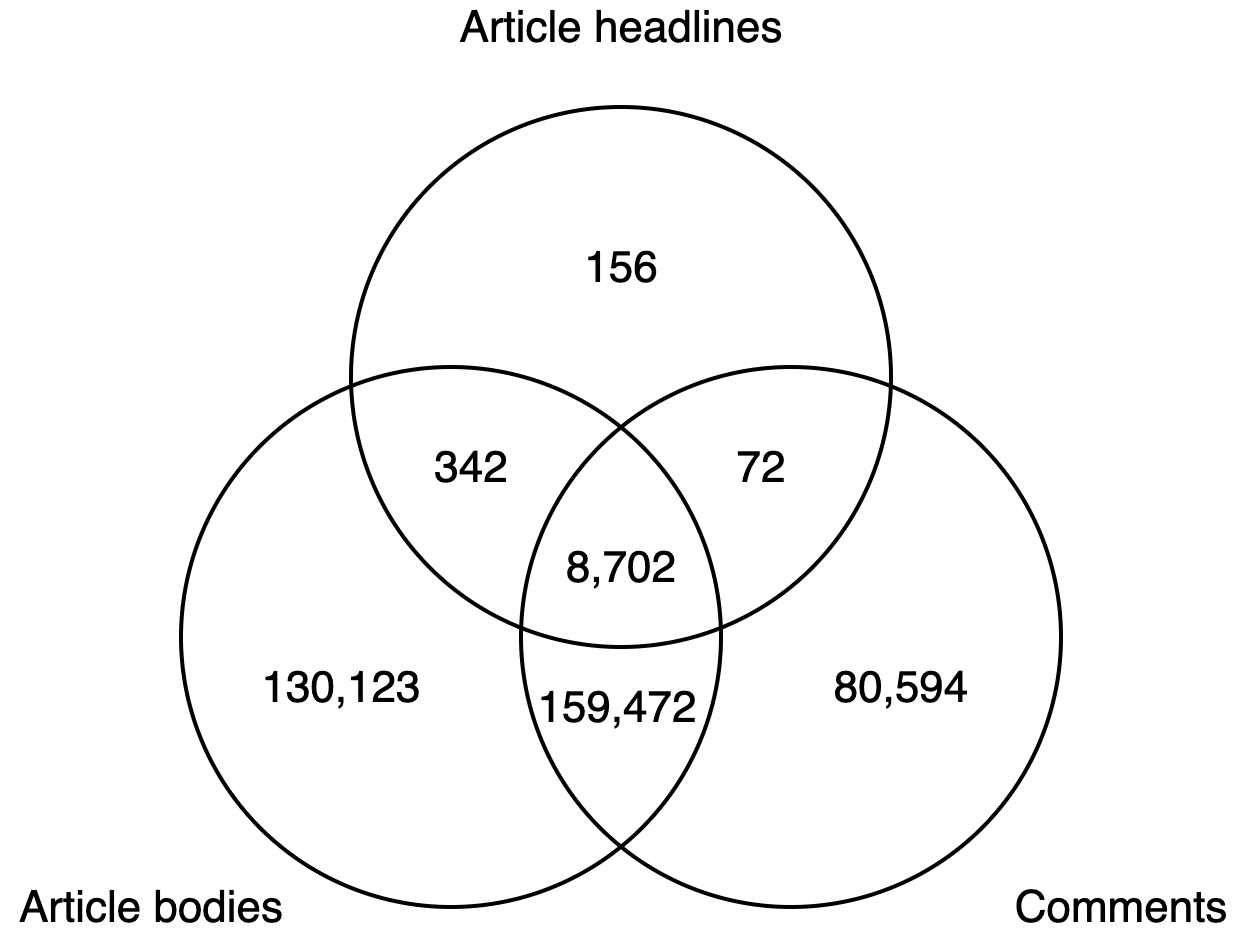
\includegraphics[scale=0.23]{0-img/vocab-venn-diagram.png}
    \caption{Venn diagram depicting overlap between each of the 3 domains in our Reddit dataset}
    \label{fig:vocab-venn-diagram}
\end{figure}
\chapter{Exploring domain adaptation techniques} \label{chap:domain-adaptation}

In this chapter we explore domain adaptation methods for detecting political bias in Reddit comments, using the cross-domain dataset developed in Chapter \ref{chap:reddit-data}. We consider a direct transfer approach, and an approach using a state-of-the-art domain-adaptive BERT model called AdaptaBERT.

\section{Notation}

Let $ A \rightarrow B $ denote some transfer from domain A to domain B, i.e. an $ A \rightarrow B $ model is a transfer learning model from source domain $ A $ to target domain $ B $. This will commonly involve training on some combination of domains A and B, and then making inferences on domain B.

We denote a standard classifier for domain $ B $ as an \textit{in-domain} model for domain $ B $ i.e. where source domain and target domain are both B (note this is \underline{not} a transfer learning model). An \textit{in-domain} model for domain B provides a theoretical upper-bound for the accuracy of an $ A \rightarrow B $ model \cite{adaptabert}, since any $ A \rightarrow B $ model will most-likely never be able to achieve the same accuracy as a model that has been trained solely on target domain B for inference on B.

\section{Direct transfer} \label{sec:direct-transfer}

\textit{Direct transfer} is the simplest form of transfer learning. An $ A \rightarrow B $ direct transfer model undergoes training solely on domain $ A $, followed by inference on domain $ B $ and appropriate evaluation metrics being recorded. A diagram of the process is shown in Figure \ref{fig:direct-transfer}.

\begin{figure}[ht]
    \centering
    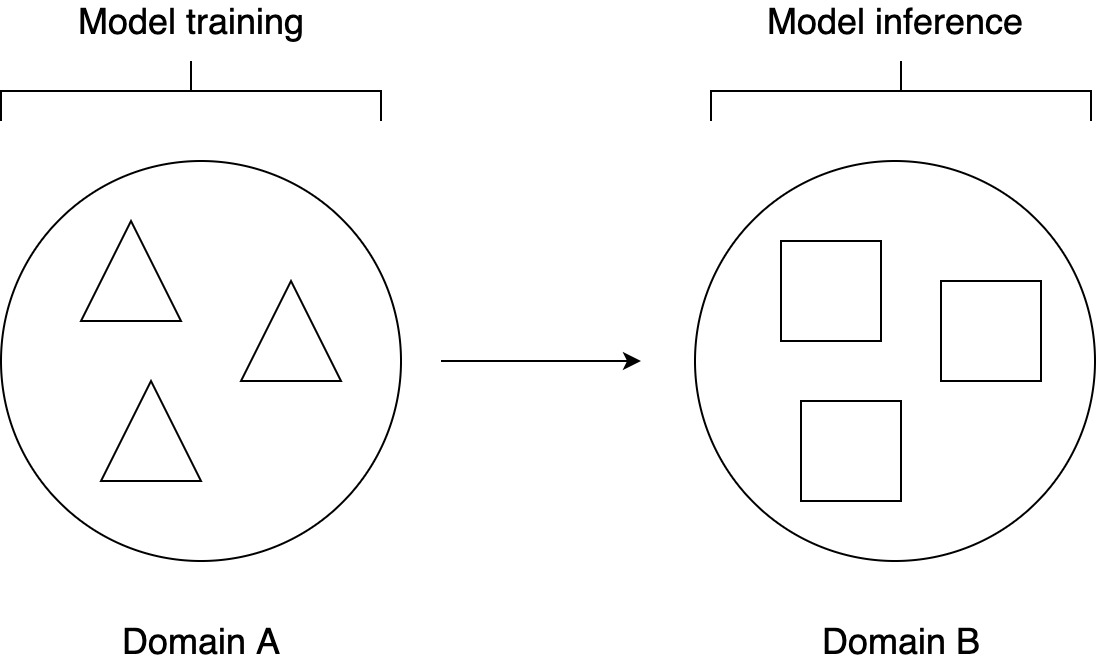
\includegraphics[scale=0.25]{0-img/direct-transfer.png}
    \caption{The direct transfer process (adapted from \cite{ruder})}
    \label{fig:direct-transfer}
\end{figure}

Using our cross-domain Reddit dataset, we will evaluate direct transfer of news articles $ \rightarrow $ comments, and also transfer of comments $ \rightarrow $ news articles. The latter is influenced by the discussion in Section \ref{sec:readership-bias} as to whether bias in the news source determines readership bias, or whether bias in the source's audience influences biases in the articles the source produces. Evaluating this transfer will help us see if audience reaction is a good predictor of news article bias. We compare these transfer models against in-domain models for articles and comments.

We use BERT sequence classification models for all of the above. With BERT direct transfer models, pre-training is performed as with standard BERT - on a large amount of English language text sourced from BookCorpus and Wikipedia. Fine-tuning is performed on the source domain, and then inference is performed on the target domain. See Figure \ref{fig:direct-transfer-in-domain-bert} for a diagram comparing direct transfer and in-domain BERT models. The training objective at each stage is shown in bold, with the domain being trained on underneath.

\begin{figure}
    \centering
    \hspace{-1.5cm}
    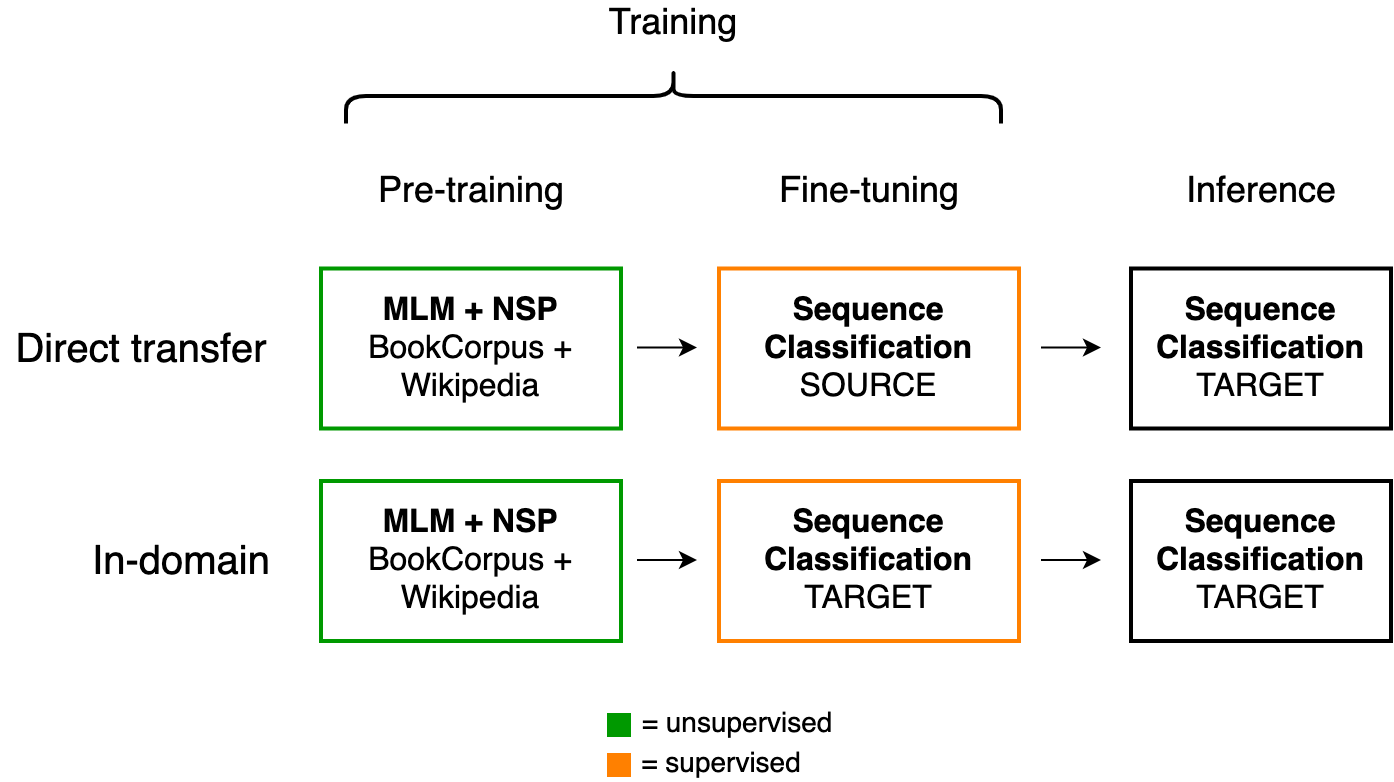
\includegraphics[scale=0.3]{0-img/direct-transfer-in-domain-bert.png}
    \caption{The stages of direct transfer and in-domain BERT approaches}
    \label{fig:direct-transfer-in-domain-bert}
\end{figure}

From Section \ref{sec:domain-similarity}, we identified 3 textual domains in our data. However, news articles can be split up into 2 domains - article headlines and article bodies. We choose to only use article bodies in our investigation, and ignore article headlines - from our results in Section \ref{subsec:nmr-bert-evaluation}, we found that using article body text to detect bias outperforms using any article headline information. From now on when we refer to `articles', we are only considering article body text.

\subsection{Experimental setup + evaluation}

We use a very similar BERT setup to our experiments in Section \ref{sec:nmr-bert}. We use a BERT model for sequence classification based on \texttt{bert-base-uncased}, and perform text preprocessing in a similar fashion. In terms of stopword removal, we use NLTK's built-in list of stopwords instead of the more minimalist approach taken earlier. For in-domain models, we use a train/validation/test split of 70:10:20. For direct transfer models, we use a 70:10:20 train/validation/test split on the source domain, after which we use the model to infer over the entire target domain. After tuning hyperparameters we achieve highest accuracies with 5 epochs of training and a batch size of 10.

We evaluate articles $ \rightarrow $ comments direct transfer against a comments in-domain model, and comments $ \rightarrow $ articles direct transfer against an articles in-domain model. We report macro-averaged F1 score and accuracy for all 4 models. Results are shown in Table \ref{tab:direct-transfer-results}.

\begin{table}[ht]
    \centering
    \begin{tabular}{|c|c|c|c|c|}
        \hline
        \textbf{Source Domain} & \textbf{Target Domain} & \textbf{Model Type} & \textbf{Macro-F1} & \textbf{Accuracy} \\
        \hline
        articles & \multirow{2}{4em}{comments} & direct transfer & 54.4 & 51.8 \\
        comments & & in-domain & 67.2 & 67.6 \\
        \hline
        comments & \multirow{2}{3em}{articles} & direct transfer & 69.6 & 69.3 \\
        articles & & in-domain & 76.2 & 76.5 \\
        \hline
    \end{tabular}
    \caption{Evaluation metrics comparing direct transfer to non-transfer baselines}
    \label{tab:direct-transfer-results}
\end{table}

We can see the direct transfer approaches are beaten by the in-domain classifiers in both F1 score and accuracy. The F1 score difference is around 13\% for articles $ \rightarrow $ comments transfer, and around 7\% for comments $ \rightarrow $ articles transfer. This suggests direct transfer by itself cannot completely substitute for training on the target domain, irrespective of which domain is the target.

The comments $ \rightarrow $ articles transfer performs significantly better than articles $ \rightarrow $ comments, both in terms of absolute metrics and in terms of how close to the in-domain baseline it is able to achieve. This suggests there is merit to the idea that looking at comments on a particular article are a good predictor for the bias of the article itself. This could be because the number of comments in our dataset is much larger than the number of articles (each article in our dataset has 14 comments on average), so the classifier has access to much more data to train on.

To test this idea, we experiment with reducing the number of comments in the dataset, and re-running the comments $ \rightarrow $ articles transfer model. Reducing the number of comments by 50\% results in an accuracy drop of around 5\%, from 69.3\% to 64.5\%, and reducing by 75\% gives a further accuracy drop of 15\%. These are significant drops in accuracy, indicating the sheer number of comments in our dataset contributes to the high accuracy of transfer.

This is an important finding, since in the real world comments are much more abundant in nature than news articles - on articles from mainstream news outlets it is common to find hundreds of comments, both on the site itself and on social media such as Facebook and Reddit. The fact that comment text is a good predictor for news article bias with only a fairly small deterioration in accuracy compared to in-domain methods is something that can be explored further in future work.

\section{AdaptaBERT} \label{sec:adaptabert}

Beyond direct transfer, more modern domain adaptation methods exploit unsupervised techniques to increase accuracy on the target domain, without needing more labelled target domain data. One such method is AdaptaBERT \cite{adaptabert}, a modified BERT architecture that is geared towards unsupervised domain adaptation.

Standard BERT models are trained for masked language modelling (MLM) and next sentence prediction (NSP) during pre-training, and then are fine-tuned for the task at hand (in our case, sequence classification). In the direct transfer case, this fine-tuning occurs only on the source domain. AdaptaBERT adds an extra fine-tuning step where another round of MLM is performed, but on a combination of the source domain and the target domain. This helps attune BERT's internal contextualised word embeddings to words in the target domain, and yields significantly better performance than direct transfer for the tasks of POS tagging and named entity recognition \cite{adaptabert}, especially on `out-of-vocabulary' (OOV) terms - words seen at inference time in the target domain that were not seen during training.

The new MLM stage is applied to a dataset containing all target domain data available, and an equal amount of source domain data (if the source domain dataset is smaller than the target domain dataset, all source domain data is used). 10 instances of each sample in this dataset are created, each with 15\% of the tokens replaced with [MASK] tokens, following the same procedure as in the original BERT paper \cite{bert}. The model is then trained to predict each masked word.

\begin{figure}[ht]
    \centering
    \hspace{-1.5cm}
    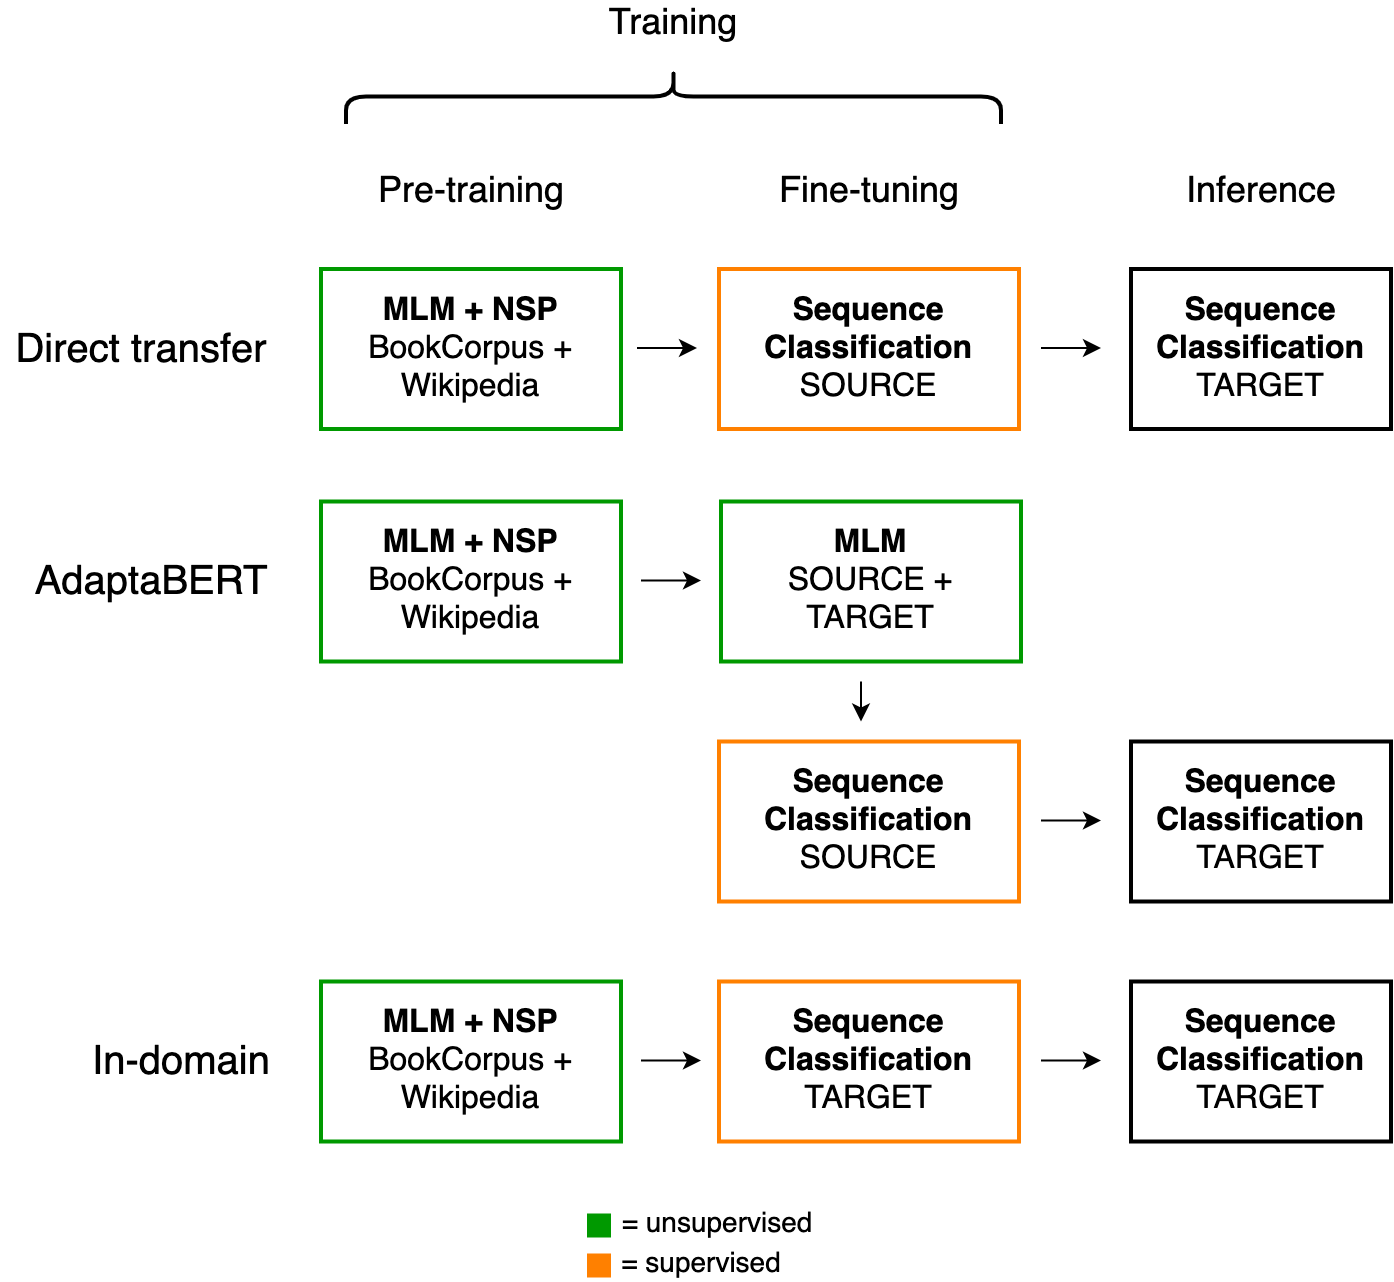
\includegraphics[scale=0.29]{0-img/adaptabert.png}
    \caption{The stages of AdaptaBERT compared to direct transfer and in-domain BERT approaches}
    \label{fig:adaptabert}
\end{figure}

A diagram comparing the AdaptaBERT approach to direct transfer and in-domain approaches is shown in Figure \ref{fig:adaptabert}. We can see AdaptaBERT only adds an extra unsupervised stage, so no extra labelled data is needed in either domain.

In Section \ref{sec:domain-similarity} we found the Jaccard distance between articles and comments in our dataset was 0.44, indicating good scope for domain adaptation due to a shared vocabulary. However, each of these domains also has a large amount of OOV terms (130,123 for articles and 80,594 for comments). Therefore, our hypothesis is that AdaptaBERT will improve classification performance dramatically over direct transfer.

\subsection{Experimental setup + evaluation} \label{subsec:adaptabert-evaluation}

We modify the code provided by the authors to run AdaptaBERT on our cross-domain Reddit dataset \cite{adaptabert-code}. The new MLM stage is very memory-intensive - we are limited to maximum sequence lengths of 128 tokens instead of the standard 512, as beyond this requires more memory than our hardware can supply. We use a learning rate of $ 5 \cdot 10^{-5} $ and a linear learning rate warm-up period of 10\% of training time as in the AdaptaBERT paper. However we find training with a batch size of 32 for 5 epochs for both the MLM and sequence classification fine-tuning tasks yields better results than the batch size of 64 for 3 epochs as used in the original paper.

Similarly to the previous section, we report results for articles $ \rightarrow $ comments transfer as well as comments $ \rightarrow $ articles transfer. We compare these against the direct transfer and in-domain baselines for the two domains from Section \ref{sec:direct-transfer}. Results are shown in Table \ref{tab:adaptabert-results} to 3.s.f.

\begin{table}[ht]
    \begin{center}
        \begin{tabular}{|c|c|c|c|c|}
            \hline
            \multicolumn{3}{|c|}{\textbf{Articles $ \rightarrow $ comments transfer}} \\
            \hline
            \textbf{Model Type} & \textbf{Macro-F1} & \textbf{Accuracy} \\
            \hline
            Direct transfer & 54.4 & 51.8  \\
            AdaptaBERT & 50.1 & 55.1 \\
            \hline
            In-domain & 67.2 & 67.6 \\
            \hline
        \end{tabular}
    \end{center} \vspace{10pt}
    \begin{center}
        \begin{tabular}{|c|c|c|}
            \hline
            \multicolumn{3}{|c|}{\textbf{Comments $ \rightarrow $ articles transfer}} \\
            \hline
            \textbf{Model Type} & \textbf{Macro-F1} & \textbf{Accuracy} \\
            \hline
            Direct transfer & 69.6 & 69.3  \\
            AdaptaBERT & 69.7 & 69.8 \\
            \hline
            In-domain & 76.2 & 76.5  \\
            \hline
        \end{tabular}
    \end{center}
    \caption{Evaluation metrics comparing AdaptaBERT to direct transfer and in-domain baselines}
    \label{tab:adaptabert-results}
\end{table}

We can see AdaptaBERT gives slightly mixed results for articles $ \rightarrow $ comments transfer, outperforming in terms of accuracy by around 4\%, however letting F1 suffer by a similar amount. In the comments $ \rightarrow $ articles case AdaptaBERT outperforms direct transfer slightly, but not in a statistically significant way. We can see in both directions, both direct transfer and AdaptaBERT fall short of the in-domain upper bound, however again the difference is much less in the comments $ \rightarrow $ articles case.

Han \& Eisenstein implement AdaptaBERT for a named entity recognition task on social media, examining transfer from news text to Twitter content \cite{adaptabert}. They find AdaptaBERT gives a 1\% improvement in F1 score over direct transfer (58.9\% vs 57.7\%), and this extends to 3\% when AdaptaBERT undergoes MLM on 1 million extra tweets. Further work could be to collect larger amounts of Reddit data and experiment running AdaptaBERT again - our Reddit dataset is fairly small, with just over 10,000 comments.

\subsection{Finding the optimal proportion of source domain examples for MLM} \label{subsec:src-proportion-adaptabert}

In standard AdaptaBERT, an equal amount of source domain and target domain examples are used for the novel MLM stage. We experiment with varying the amount of source domain content used relative to target domain content to see if we can improve classifier accuracy.

We evaluate AdaptaBERT for both article $ \rightarrow $ comment transfer and comment $ \rightarrow $ article tranfer, with source proportion values of 0, 1/3, 2/3 and 1 (where `source proportion' = number of source domain examples as a proportion of target domain examples). For each experiment we always use all target domain data available. Results are shown in Figure \ref{fig:src-proportion}.

\begin{figure}[ht]
    \centering
    \begin{subfigure}{\textwidth}
        \centering
        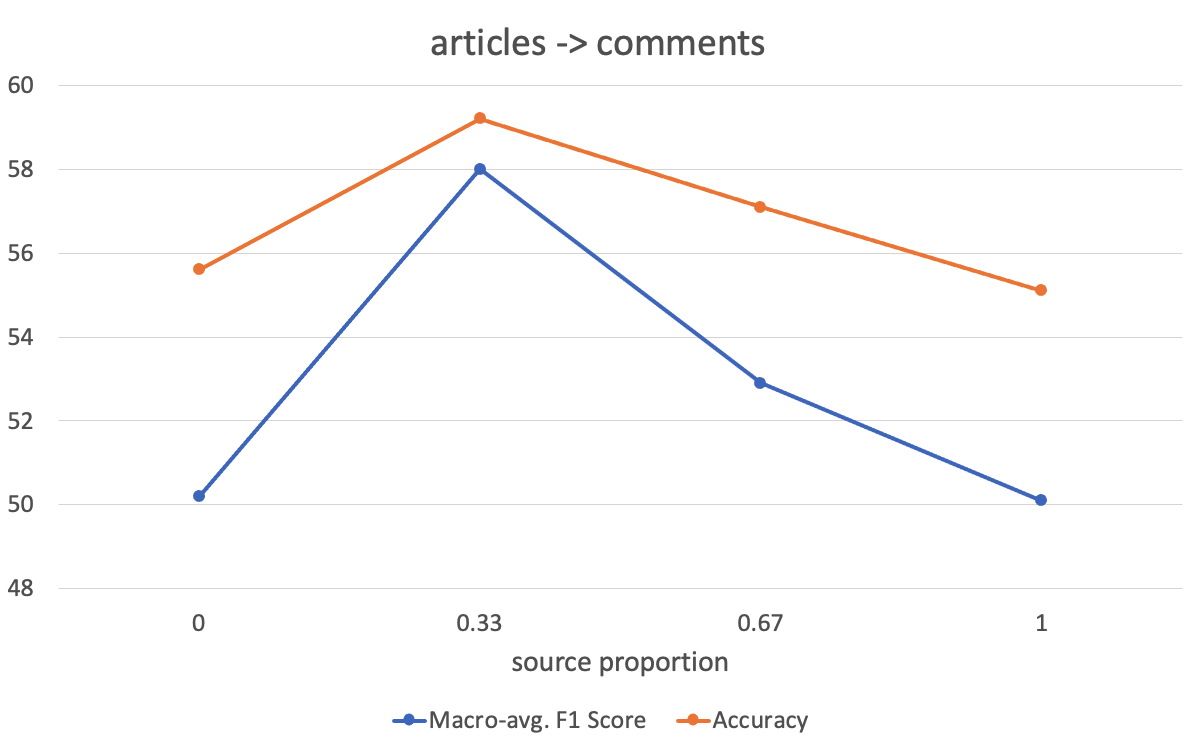
\includegraphics[scale=0.3]{0-img/src-proportion-articles-comments.png}
    \end{subfigure}
    \begin{subfigure}{\textwidth}
        \centering
        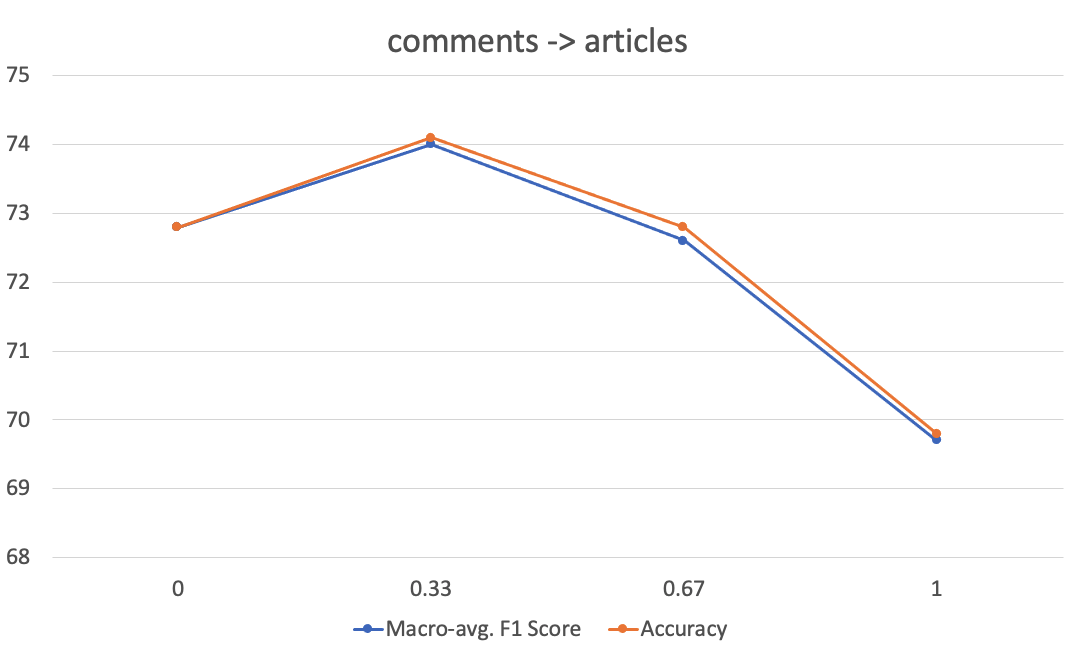
\includegraphics[scale=0.3]{0-img/src-proportion-comments-articles.png}
    \end{subfigure}
    \caption{Performance of AdaptaBERT when varying proportion of source domain examples compared to target domain examples used in the MLM stage}
    \label{fig:src-proportion}
\end{figure}

We can see for both directions of transfer, using 1/3 of the number of target domain examples for the source domain provides the both the best F1 score and accuracy. Compared to using an equal amount of source and target domain examples (a source proportion of 1), this boosts F1 scores by \textasciitilde 8\% to 58.0\% for articles $ \rightarrow $ comments transfer and by \textasciitilde 4\% to 74.0\% for comments $ \rightarrow $ articles transfer. This is a significant improvement over the results in Table \ref{tab:adaptabert-results}. Note that in the comments $ \rightarrow $ articles case, this puts us only a few \% short of the in-domain baseline.

There is a general trend of increasing deterioration in classification performance the more source domain material is added to the MLM stage - this shows us classification performance is highest when the amount of source domain material used is fairly low compared to target domain material. This makes sense, since after a point adding more source domain material could attune BERT's internal contextualised embeddings too much towards source domain material, and could cause it to start `forgetting' some target domain context. This is linked to a wider problem in neural-network-based models called `catastrophic forgetting' \cite{catastrophic-forgetting}. 
\chapter{Extending AdaptaBERT with Next Sentence Prediction} \label{chap:extending-adaptabert}

Having described the AdaptaBERT model and measured its performance for the political bias detection task on our cross-domain Reddit dataset, we now extend AdaptaBERT by adding a Next Sentence Prediction stage to its fine-tuning stages, and assess the performance of the new model on political bias detection and named entity recognition tasks.

\section{Motivation}

Currently, AdaptaBERT only adds an extra masked language modelling objective to the training stages of BERT. However, standard BERT undergoes two pretraining objectives to train its contextualised word embeddings - masked language modelling (MLM) and next sentence prediction (NSP). The original BERT paper \cite{bert} states that the MLM objective is used to train a deep bidirectional internal representation of the words, and NSP is used mainly to help improve BERT's performance on question answering and natural language inference tasks.

Intuitively this makes sense - tuning BERT's internal representations to better understand context between sentences will help it perform better at tasks which require scanning long sequences of text, such as QA and NLI. However, our cross-domain dataset of articles and Reddit comments also contains samples with long text sequences - each article in our dataset contains 31 sentences on average. Comments are less sentence-heavy, with each comment containing on average 2 sentences. Both domains show heavy right-hand skew in the distribution of number of sentences (see Figure \ref{fig:num-sentences-distributions}).

\begin{figure}[ht]
    \centering
    \begin{subfigure}{\textwidth}
        \centering
        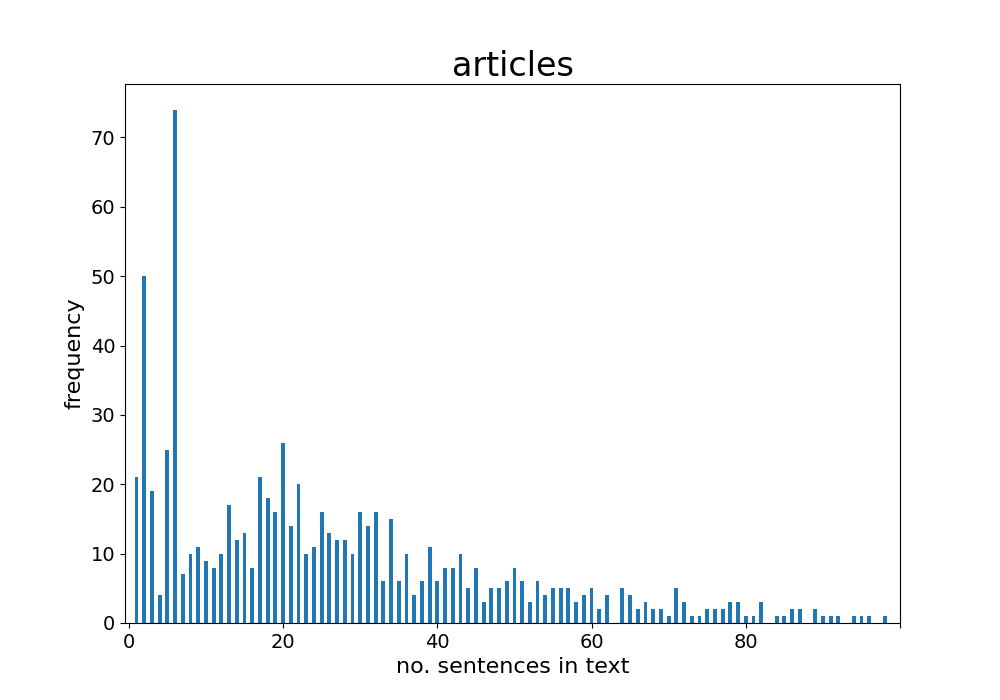
\includegraphics[scale=0.45]{0-img/num-sentences-distribution-articles.png}
    \end{subfigure}
    \begin{subfigure}{\textwidth}
        \centering
        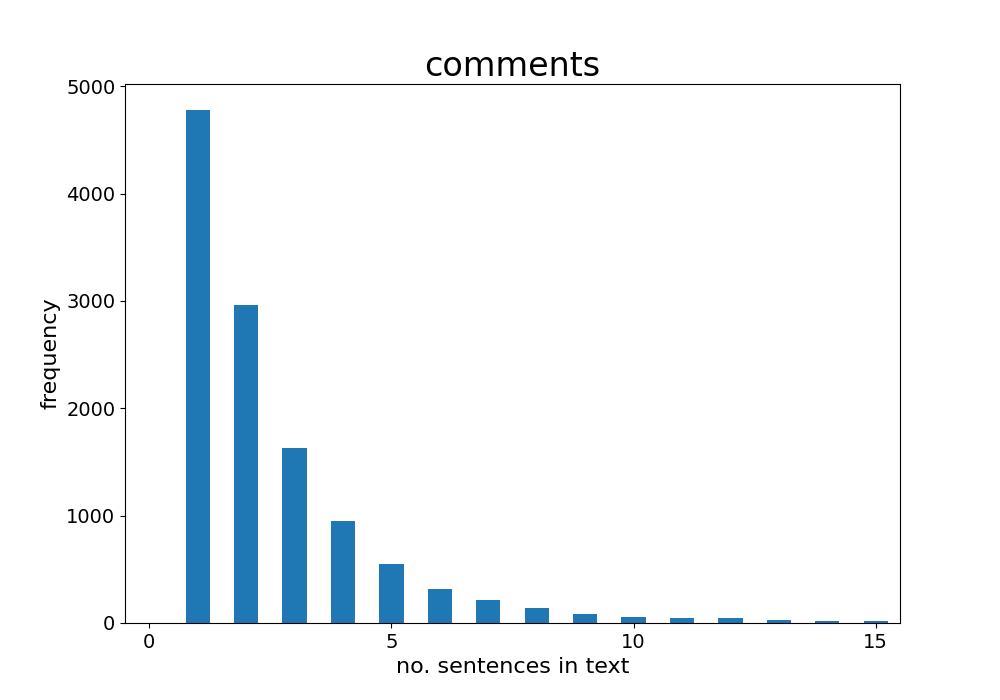
\includegraphics[scale=0.45]{0-img/num-sentences-distribution-comments.png}
    \end{subfigure}
    \caption{Distribution of number of sentences in each article (top) and comment (bottom) in our Reddit dataset}
    \label{fig:num-sentences-distributions}
\end{figure}

We explore extending AdaptaBERT by adding a Next Sentence Prediction stage directly after the MLM stage, to see if this improves classification performance. Our hypothesis is that this will improve performance in the comments $ \rightarrow $ articles scenario, since in this case the target domain contains textual content with many sentences per sample (31 on average), however the performance benefit will not be so great for articles $ \rightarrow $ comments, since the target domain in this case doesn't exhibit many sentences per sample. The architecture we propose is shown in Figure \ref{fig:adaptabert-nsp}, compared against standard AdaptaBERT and previous approaches. We call this extended model \textbf{AdaptaBERT++}. 

\begin{figure}
    \centering
    \hspace{-1.5cm}
    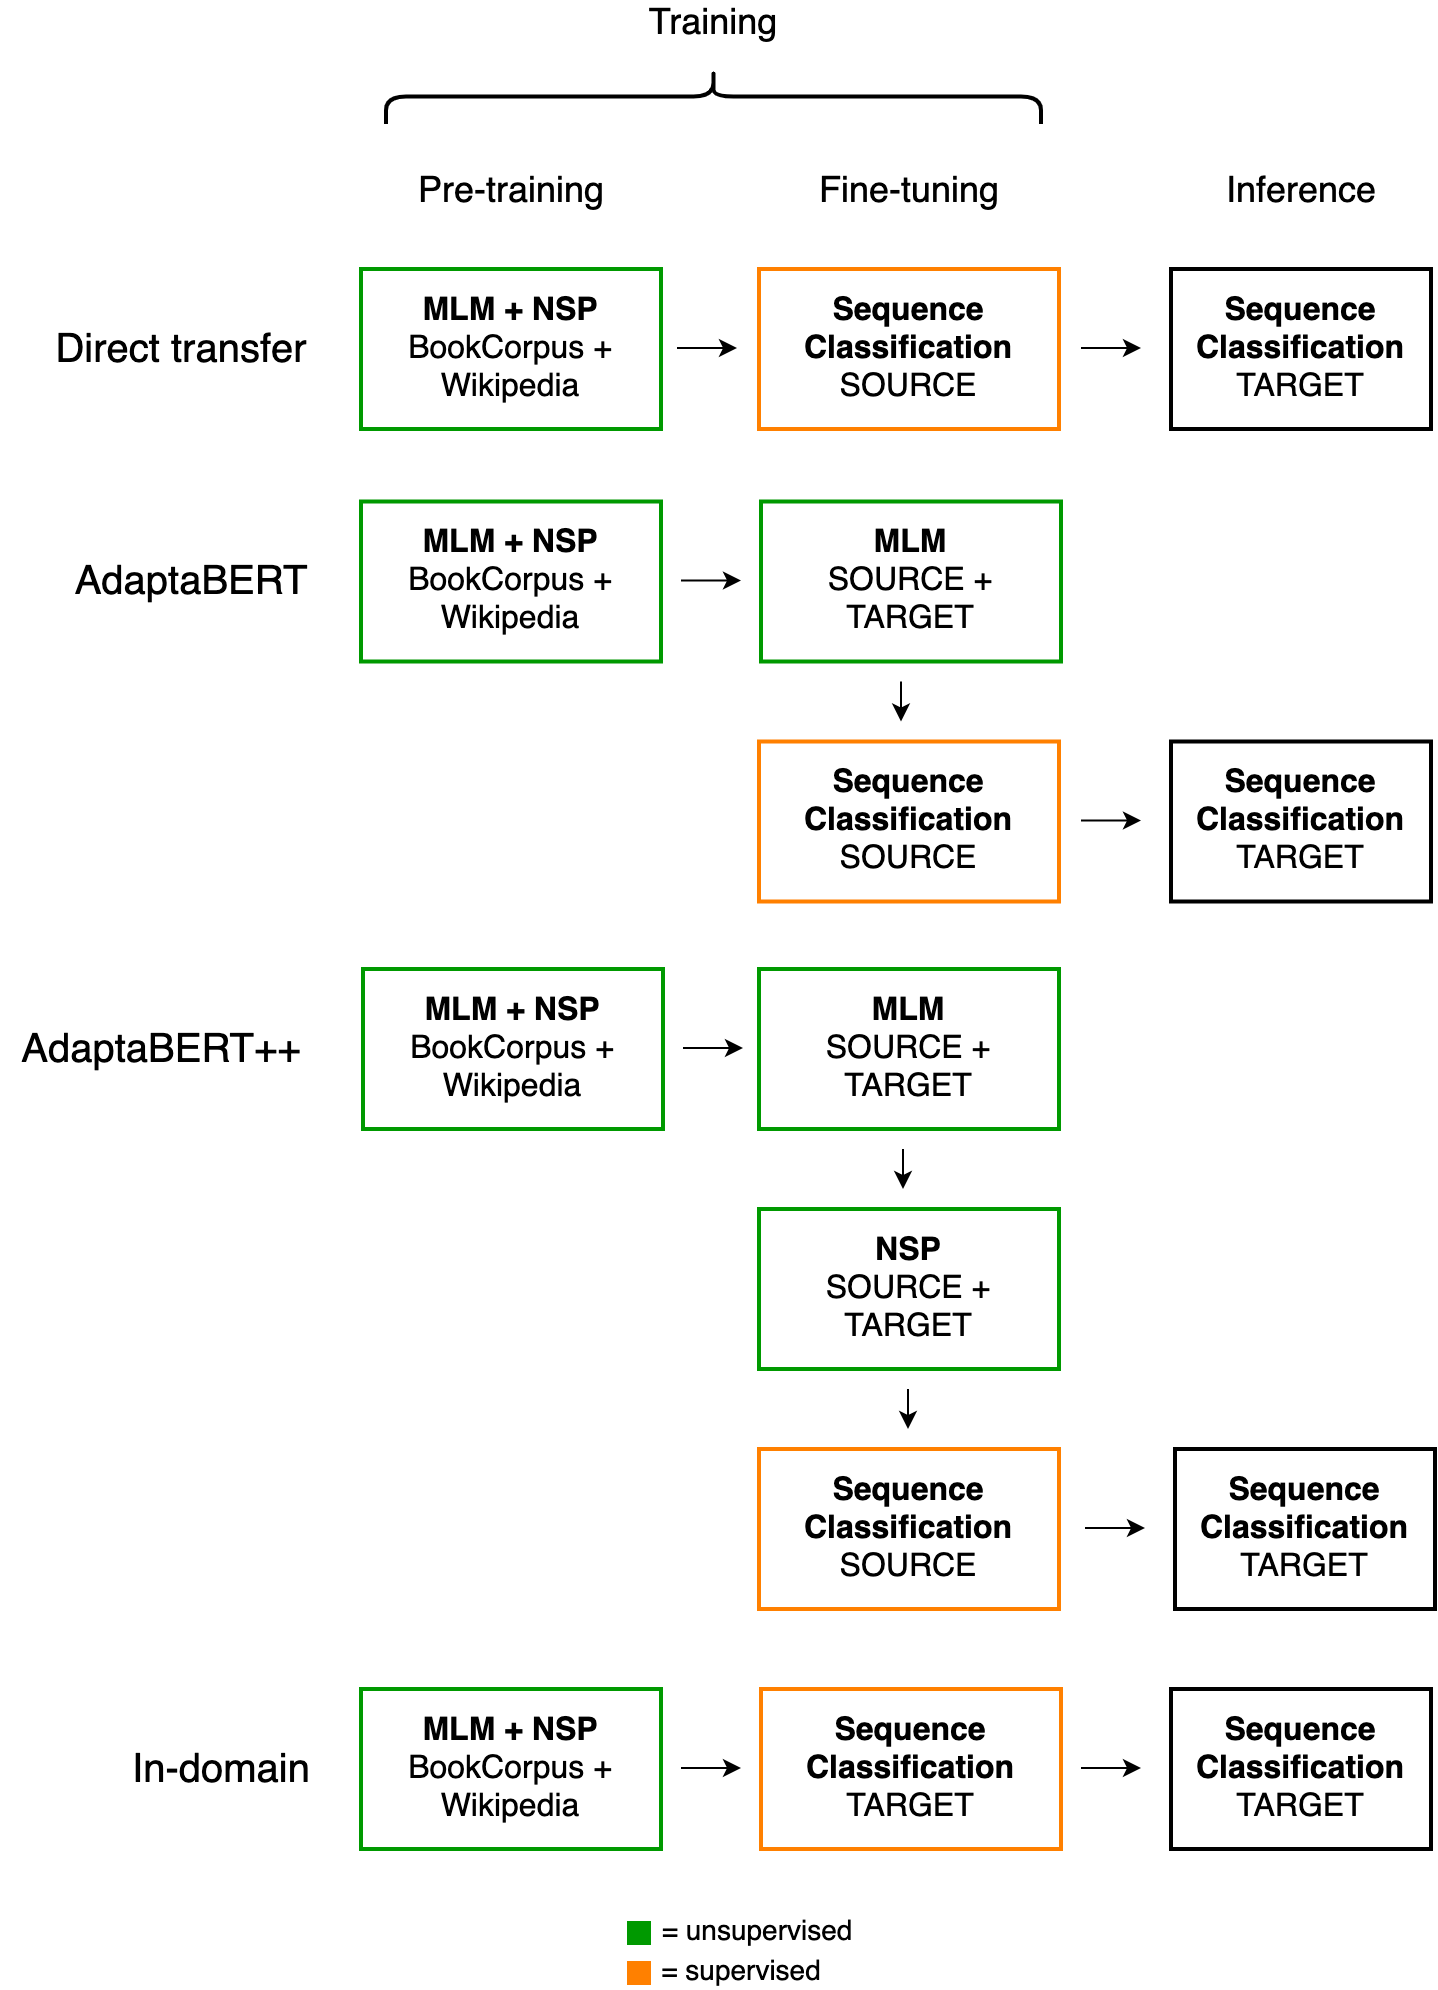
\includegraphics[scale=0.28]{0-img/adaptabert-nsp.png}
    \caption{AdaptaBERT extended with the NSP stage (AdaptaBERT++), compared to standard AdaptaBERT, direct transfer and in-domain approaches}
    \label{fig:adaptabert-nsp}
\end{figure}

\section{Implementing next sentence prediction}

In the original BERT paper \cite{bert}, NSP is implemented by creating sentence pair examples \texttt{<A, B>} out of the pre-training corpus where 50\% of the time sentence B is actually the sentence that follows A in the corpus, and the other 50\% of the time it is a randomly-selected sentence. BERT is then trained for a binary classification objective to determine for each sentence pair whether sentence B actually follows sentence A or not. We mirror this methodology for AdaptaBERT++.

Similarly to standard AdaptaBERT, we use an equal amount of source domain and target domain examples in the NSP stage, up to a maximum of the entire target domain. For each article and comment in our dataset, we choose 2 sentence pairs where the second sentence actually follows the first sentence, and 2 pairs where the second sentence is instead a random sentence from the same text. This gives us a collection of NSP training examples 4x larger than the size of the target domain.

\section{Experimental setup}

We compare the performance of AdaptaBERT++ to standard AdaptaBERT in two scenarios - political bias detection with the Reddit dataset as we have been doing previously, and also the named entity recognition (NER) task explored by Han \& Eisenstein in the original AdaptaBERT paper \cite{adaptabert}.

The NER task is an example of a token classification task - so far, we have only explored sequence classification for political bias detection. Han \& Eisenstein explore transfer from news content to tweets, using the CoNLL-2003 and WNUT 2016 NER datasets. The CoNLL dataset \cite{conll} is a corpus of 1,393 Reuters news stories \cite{reuters} taken between August 1996 and August 1997, and the WNUT NER dataset \cite{wnut} (taken from the Workshop of Noisy User Text 2016) is a collection of 3,819 generic tweets sampled from between December 2014 and February 2015. Both datasets are annotated at the token level by named entity (e.g. company, person, TV show, etc).

When tuning hyperparameters, we achieve best performance on both tasks when using only 1 epoch for the NSP stage. We use 5 epochs for MLM and sequence classification fine-tuning, as in Section \ref{sec:adaptabert}. We also use a source proportion of 1/3 for the MLM stage, as we found in Section \ref{subsec:src-proportion-adaptabert} that this gives the best performance for standard AdaptaBERT.

\section{Evaluation for political bias detection task}

As in Chapter \ref{chap:domain-adaptation}, we report results for both articles $ \rightarrow $ comments transfer and comments $ \rightarrow $ articles transfer. Results are shown in Table \ref{tab:adaptabert-nsp-results}.

\begin{table}[ht]
    \begin{center}
        \begin{tabular}{|c|c|c|c|c|c|}
            \hline
            \multicolumn{3}{|c|}{\textbf{Task}} & \multicolumn{3}{|c|}{Bias detection} \\
            \hline
            \multicolumn{3}{|c|}{\textbf{Transfer direction}} & \multicolumn{3}{|c|}{Articles $ \rightarrow $ comments} \\
            \hline \hline
            \multicolumn{2}{|c|}{\textbf{Model Type}} & \multicolumn{2}{|c|}{\textbf{Macro-F1}} & \multicolumn{2}{|c|}{\textbf{Accuracy}} \\
            \hline
            \multicolumn{2}{|c|}{Direct transfer} & \multicolumn{2}{|c|}{54.4} & \multicolumn{2}{|c|}{51.8} \\
            \multicolumn{2}{|c|}{AdaptaBERT} & \multicolumn{2}{|c|}{50.1} & \multicolumn{2}{|c|}{55.1} \\
            \multicolumn{2}{|c|}{AdaptaBERT++} & \multicolumn{2}{|c|}{58.0} & \multicolumn{2}{|c|}{58.1} \\
            \hline
            \multicolumn{2}{|c|}{In-domain} & \multicolumn{2}{|c|}{67.2} & \multicolumn{2}{|c|}{67.6} \\
            \hline
        \end{tabular}
    \end{center} \vspace{10pt}
    \begin{center}
        \begin{tabular}{|c|c|c|c|c|c|}
            \hline
            \multicolumn{3}{|c|}{\textbf{Task}} & \multicolumn{3}{|c|}{Bias detection} \\
            \hline
            \multicolumn{3}{|c|}{\textbf{Transfer direction}} & \multicolumn{3}{|c|}{Comments $ \rightarrow $ articles} \\
            \hline \hline
            \multicolumn{2}{|c|}{\textbf{Model Type}} & \multicolumn{2}{|c|}{\textbf{Macro-F1}} & \multicolumn{2}{|c|}{\textbf{Accuracy}} \\
            \hline
            \multicolumn{2}{|c|}{Direct transfer} & \multicolumn{2}{|c|}{69.6} & \multicolumn{2}{|c|}{69.3}  \\
            \multicolumn{2}{|c|}{AdaptaBERT} & \multicolumn{2}{|c|}{69.7} & \multicolumn{2}{|c|}{69.8} \\
            \multicolumn{2}{|c|}{AdaptaBERT++} & \multicolumn{2}{|c|}{70.9} & \multicolumn{2}{|c|}{71.0} \\
            \hline
            \multicolumn{2}{|c|}{In-domain} & \multicolumn{2}{|c|}{76.2} & \multicolumn{2}{|c|}{76.5}  \\
            \hline
        \end{tabular}
    \end{center}
    \caption{Evaluation metrics comparing AdaptaBERT++ to AdaptaBERT, direct transfer and in-domain baselines for political bias detection task}
    \label{tab:adaptabert-nsp-results}
\end{table}

We can see in the articles $ \rightarrow $ comments case AdaptaBERT++ improves over standard AdaptaBERT by 8\% in F1 score and 3\% in accuracy. However, in the comments $ \rightarrow $ articles case AdaptaBERT++ does not significantly outperform standard AdaptaBERT. This is not what we were expecting - our hypothesis was that adding NSP would improve classification performance when the target domain is the domain with more sentences per example (i.e. when articles is the target domain), however AdaptaBERT++ actually improves accuracy when comments is the target domain. We can infer from this that NSP appears to help transfer when the source domain is the one with more sentences per example, rather than target domain, however ideally more experiments on different datasets are needed to validate this.

\section{Evaluation for NER task}

We only evaluate articles $ \rightarrow $ tweets transfer, since this is the only transfer direction evaluated by Han \& Eisenstein \cite{adaptabert}. They also only provide F1 score and not accuracy. Results are shown in Table \ref{tab:adaptabert-nsp-ner-results}.

\begin{table}[ht]
    \begin{center}
        \begin{tabular}{|c|c|}
            \hline
            \textbf{Task} & NER \\
            \hline
            \textbf{Transfer direction} & Articles $ \rightarrow $ tweets \\
            \hline \hline
            \textbf{Model Type} & \textbf{Macro-F1} \\
            \hline
            Direct transfer & 57.7  \\
            AdaptaBERT & 58.9  \\
            AdaptaBERT++ & 61.4  \\
            \hline
            In-domain & 64.3 \\
            \hline
        \end{tabular}
    \end{center}
    \caption{Evaluation metrics comparing AdaptaBERT++ to AdaptaBERT, direct transfer and in-domain baselines for NER task. Results 1, 2, and 4 taken from \cite{adaptabert}.}
    \label{tab:adaptabert-nsp-ner-results}
\end{table}

We can see AdaptaBERT++ improves over AdaptaBERT by 2.5\% in F1 score, and comes within 3\% of the in-domain baseline.

Examining the distribution of sentences in the NER dataset (see Figure \ref{fig:ner-num-sentences-distributions}), we can see in fact both domains exhibit a low number of sentences per example. The articles, rather than having been preserved as single examples, have been split up into roughly 1 sentence per example by the WNUT dataset authors. A minority of examples contain 2 or more sentences. The average number of sentences in each tweet is of course quite low, due to Twitter's 140-character tweet limit as of December 2016, the month the dataset was published.

\begin{figure}[ht]
    \centering
    \begin{subfigure}{\textwidth}
        \centering
        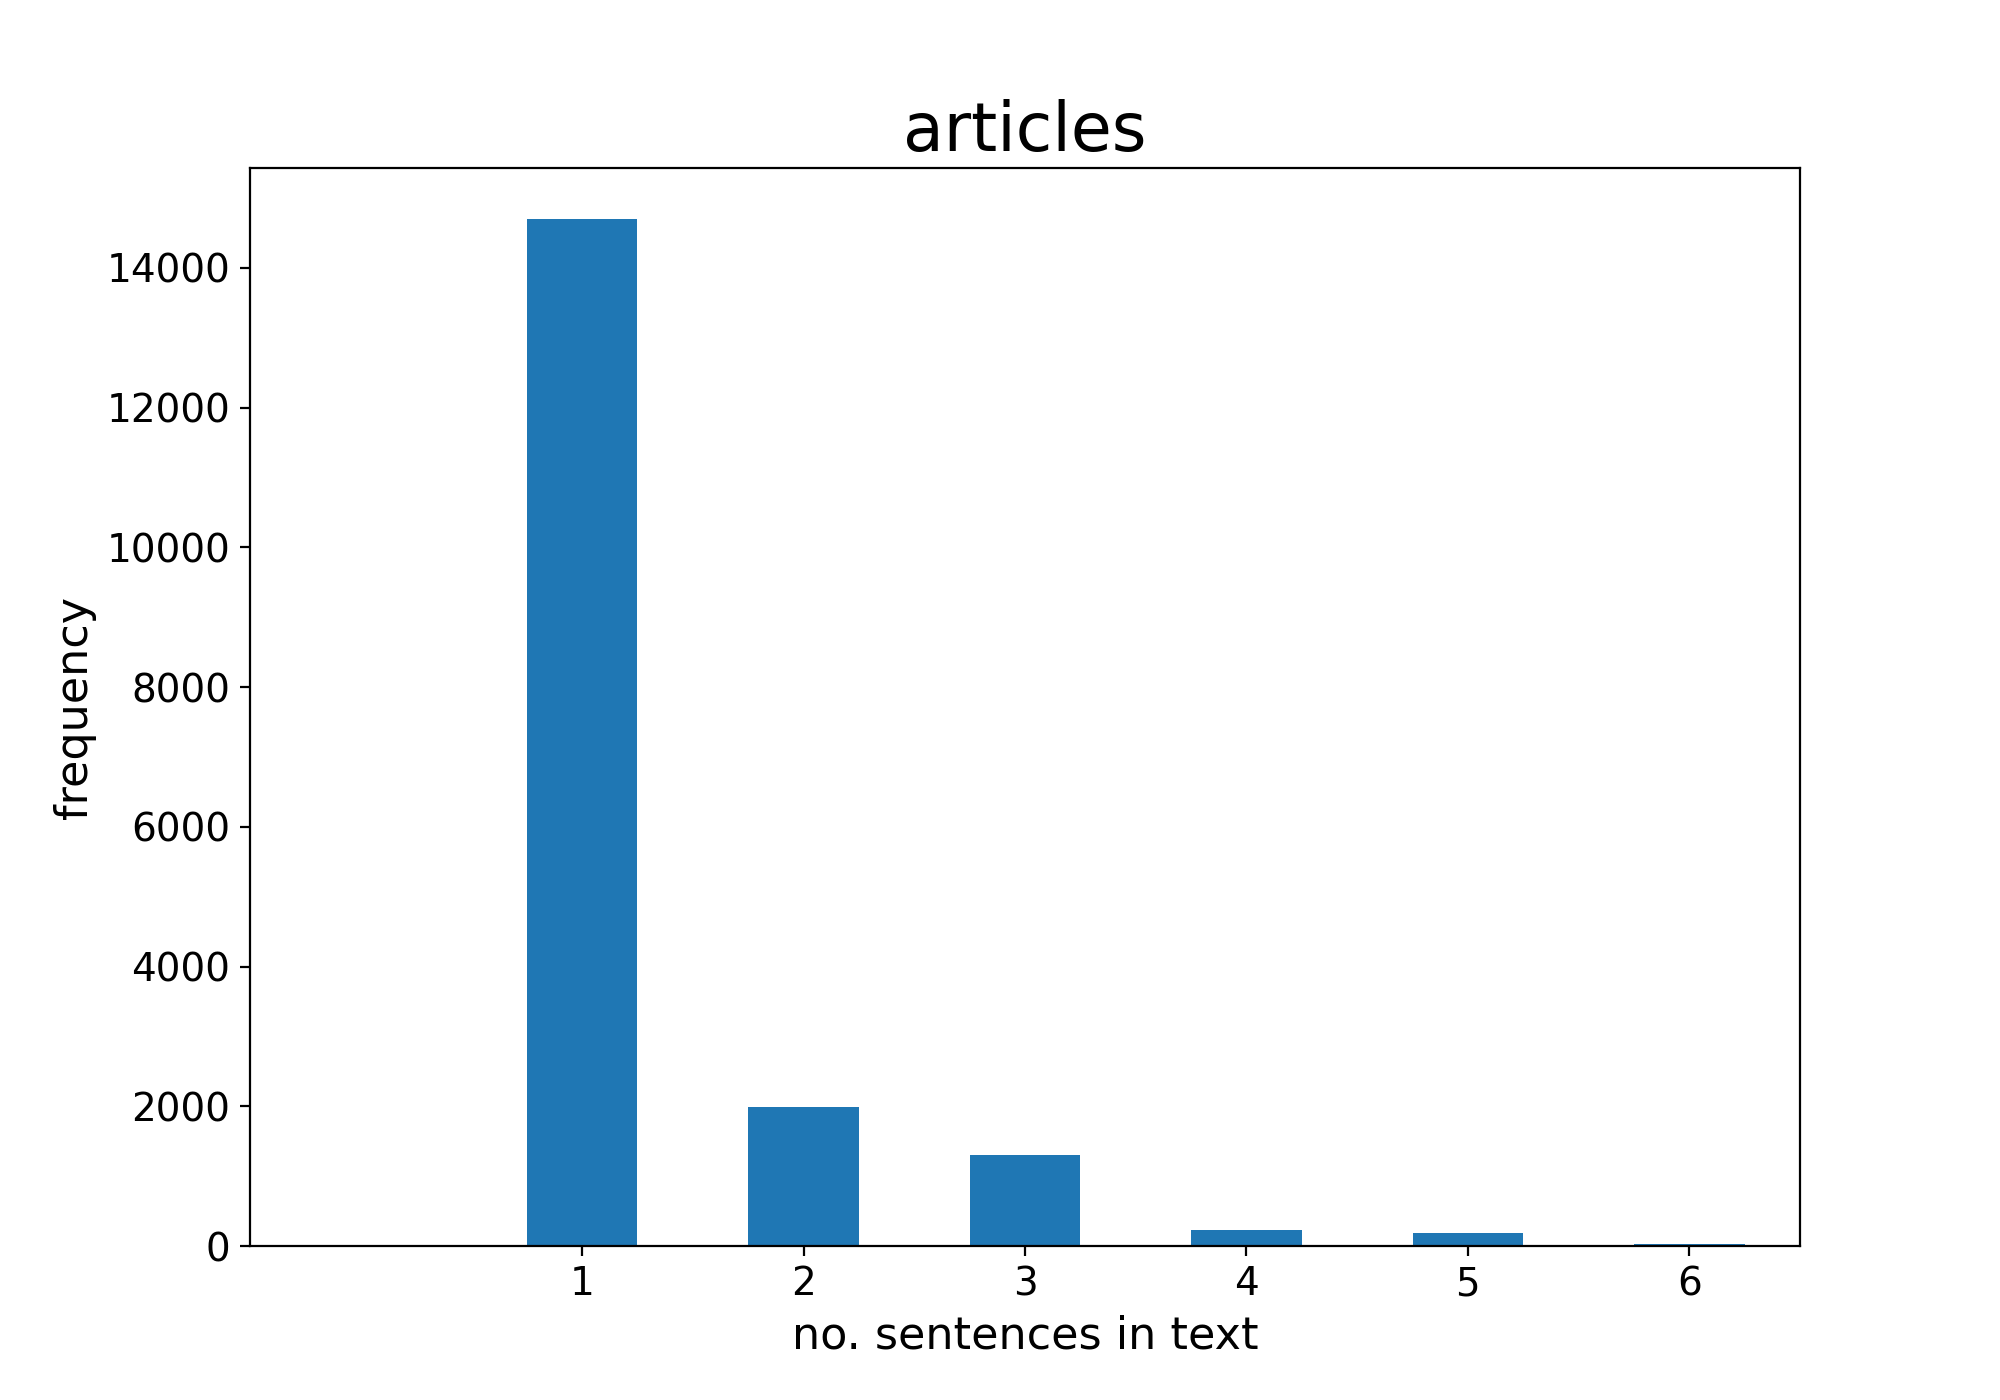
\includegraphics[scale=0.45]{0-img/ner-num-sentences-distribution-articles.png}
    \end{subfigure}
    \begin{subfigure}{\textwidth}
        \centering
        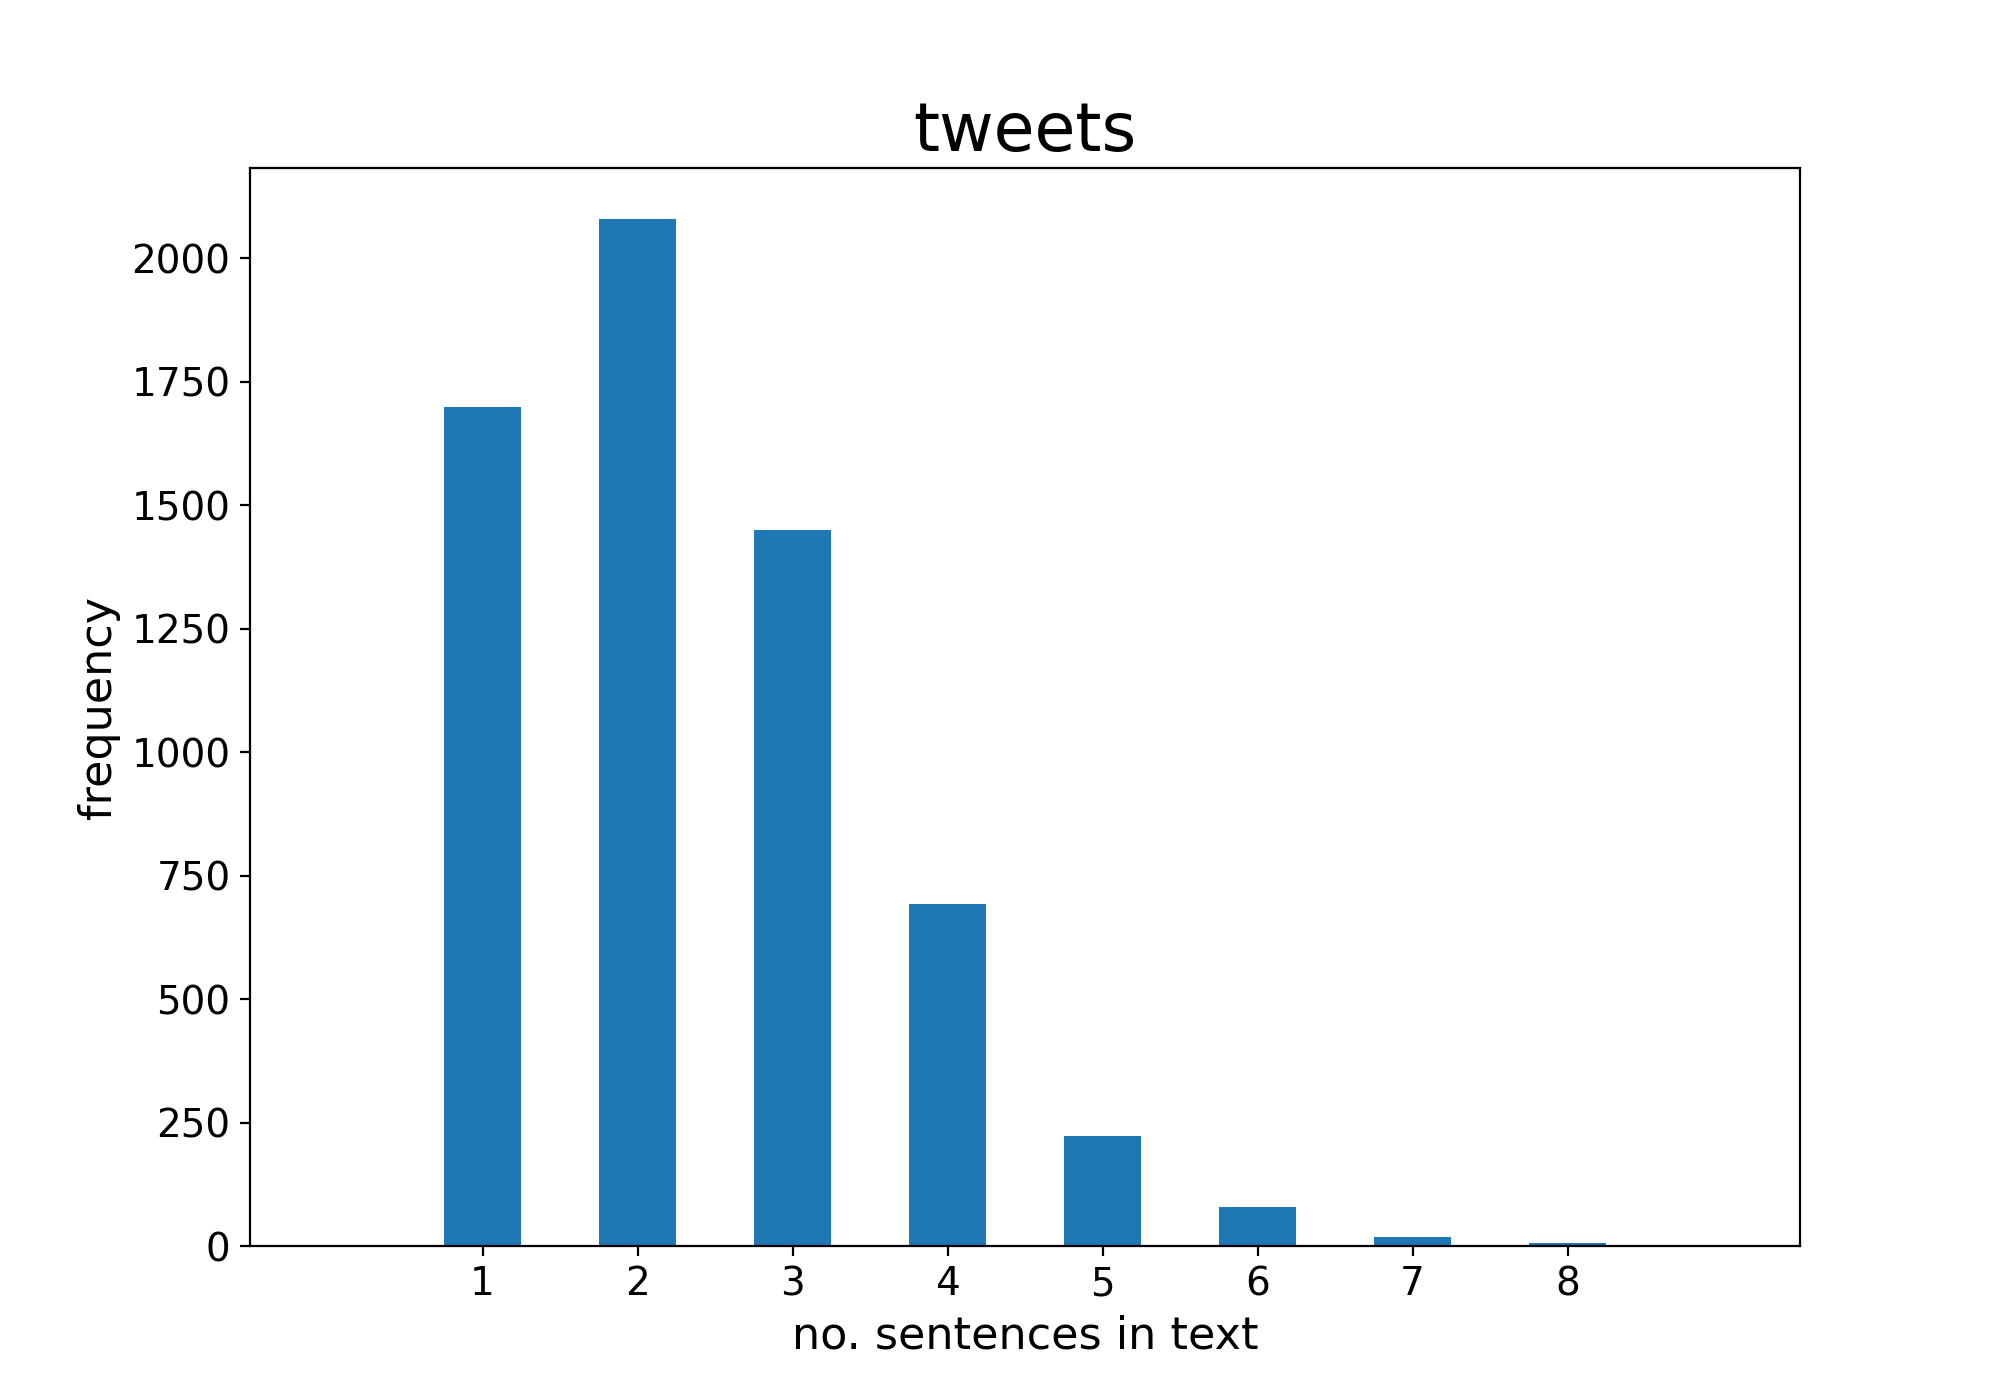
\includegraphics[scale=0.45]{0-img/ner-num-sentences-distribution-tweets.png}
    \end{subfigure}
    \caption{Distribution of number of sentences in each article (top) and tweet (bottom) in the WNUT 2016 NER dataset}
    \label{fig:ner-num-sentences-distributions}
\end{figure}

This shows us that AdaptaBERT++ can still improve over standard AdaptaBERT even when both the source and target domain exhibit a low number of sentences per training example, albeit the improvement is less than for the political bias detection task, where we were seeing improvements in F1 score of up to 8\%.

As mentioned in Section \ref{subsec:adaptabert-evaluation}, Han \& Eisenstein extend their MLM training corpus with an extra 1 million unlabeled tweets, which provides an extra boost in performance. Further work can be done evaluating AdaptaBERT++ with a larger scale cross-domain Reddit dataset.

\section{Finding the optimal proportion of source domain examples for NSP}

In the previous sections, we used an equal number of source and target domain examples for the Next Sentence Prediction stage. We now aim to find which ratio of source to target domain examples gives the optimal performance of AdaptaBERT++, similarly to our experiments with the MLM stage in standard AdaptaBERT in Section \ref{subsec:src-proportion-adaptabert}. We will use our cross-domain Reddit dataset for this set of experiments.

Again, we trial source proportion values of 0, 1/3, 2/3 and 1. In all cases we use all target domain data available. Results are shown in Figure \ref{fig:ner-src-proportion}.

\begin{figure}[ht]
    \centering
    \begin{subfigure}{\textwidth}
        \centering
        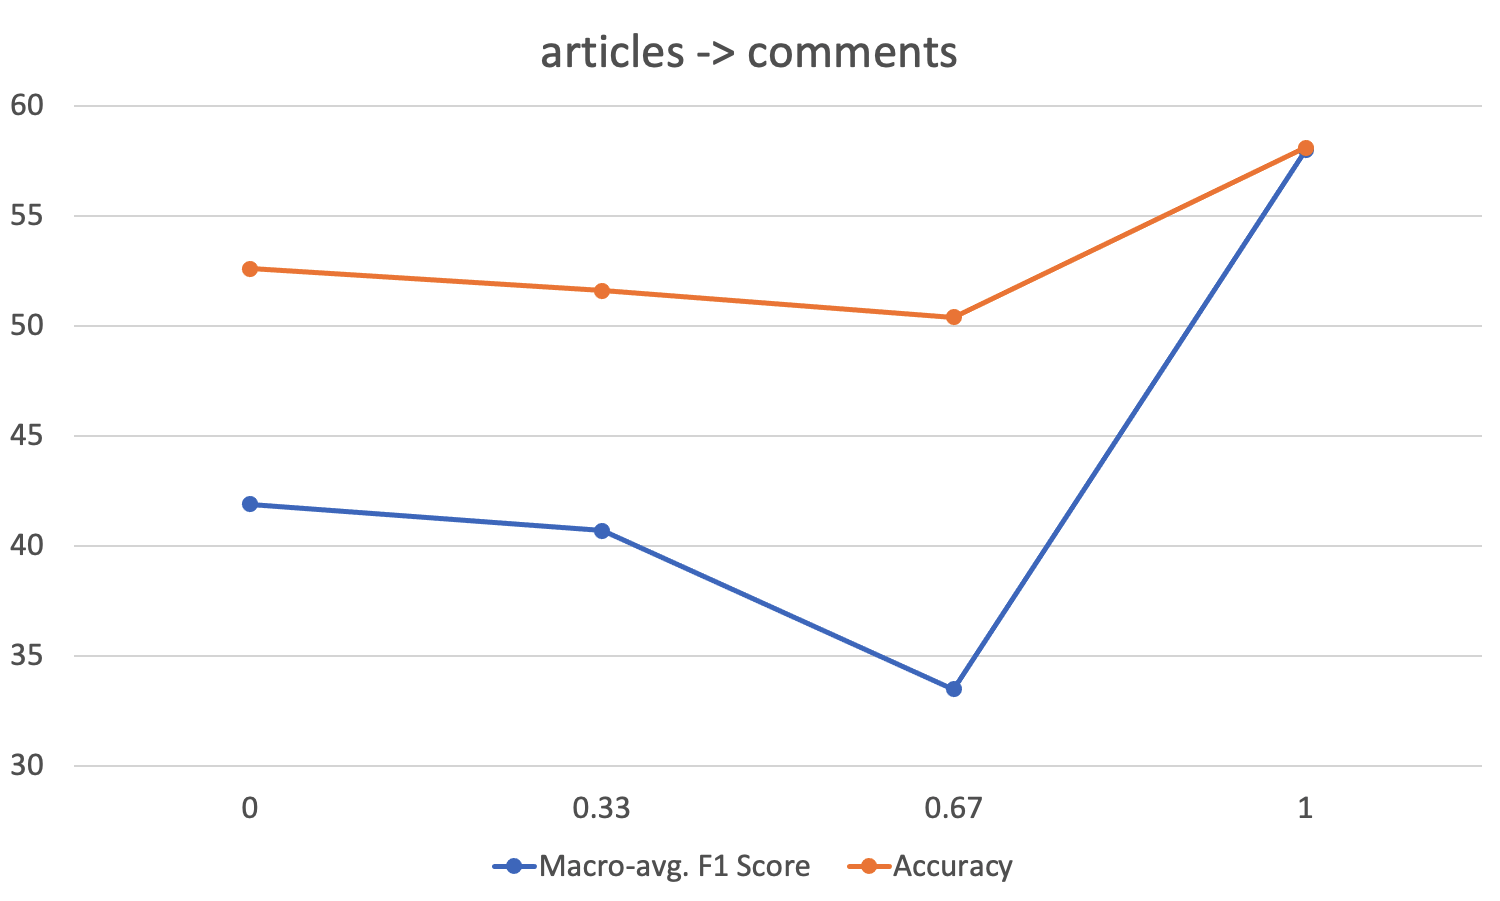
\includegraphics[scale=0.24]{0-img/ner-src-proportion-articles-comments.png}
    \end{subfigure}
    \begin{subfigure}{\textwidth}
        \centering
        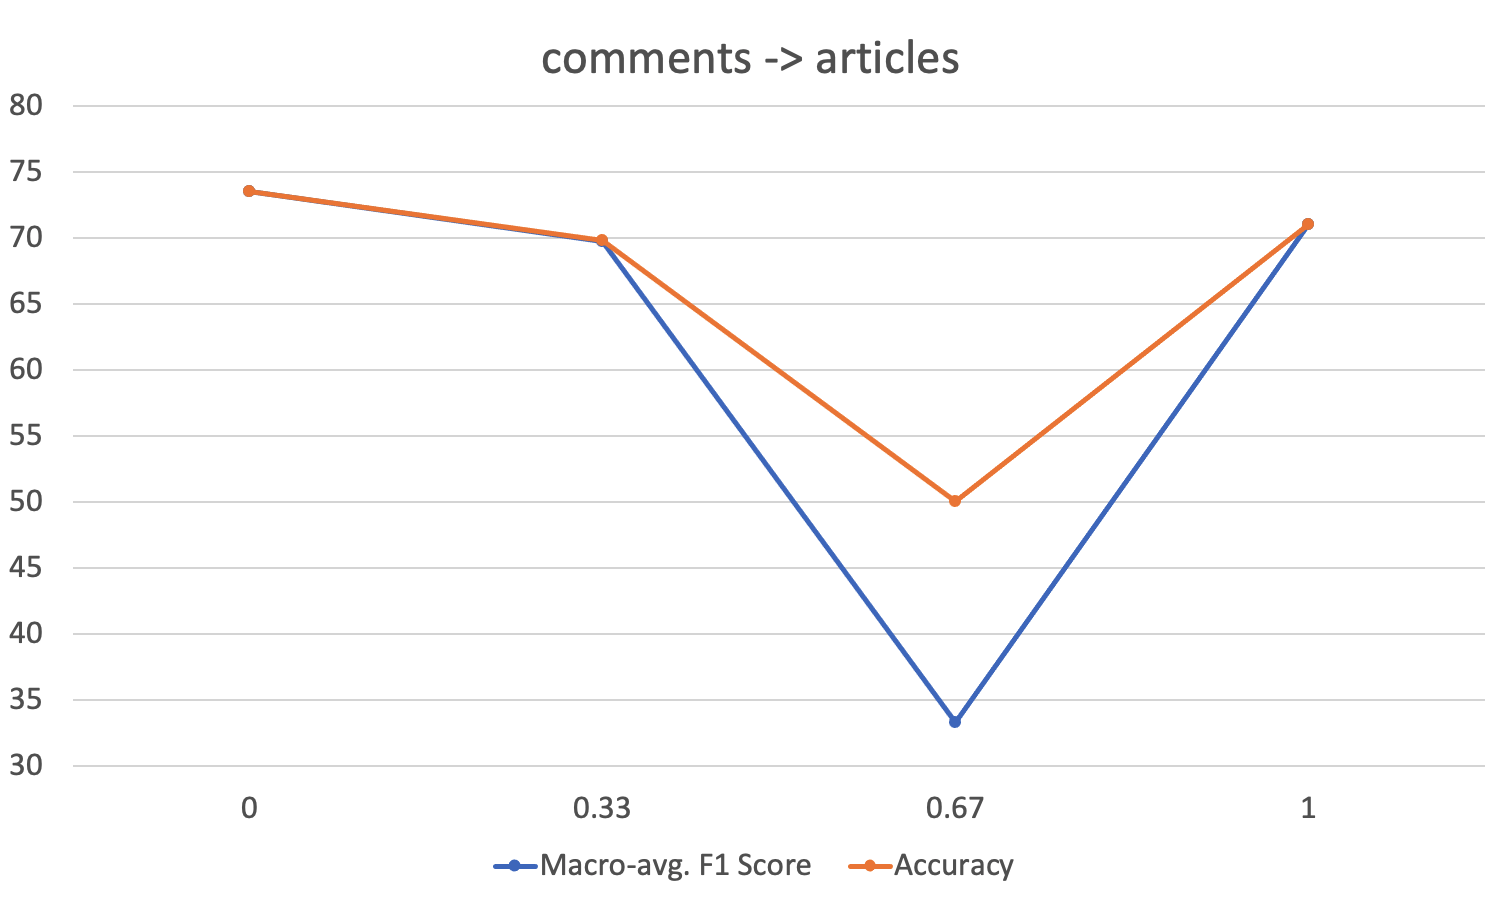
\includegraphics[scale=0.24]{0-img/ner-src-proportion-comments-articles.png}
    \end{subfigure}
    \caption{Performance of AdaptaBERT++ when varying proportion of source domain examples compared to target domain examples used in the NSP stage}
    \label{fig:ner-src-proportion}
\end{figure}

We can see in the articles $ \rightarrow $ comments case we achieve the best metrics with a source proportion of 1 (i.e. using an equal amount of source and target domain data). Interestingly, in the comments $ \rightarrow $ articles case we achieve the best metrics using no source domain material at all in the NSP stage (the F1 line is hidden behind the accuracy line between source proportions of 0 and 1/3). These results don't follow the same pattern seen in Section \ref{subsec:src-proportion-adaptabert}, where adding more source domain material leads to increasing deterioration in model performance. In fact, in both transfer directions using an equal amount of source and target domain material in the NSP stage results in very good classifier performance compared to other ratios.
\chapter{Conclusion, Evaluation, Ethical Issues \& Future Work}

\section{Conclusion}



\section{Evaluation}

Reddit subreddit titles (which form our annotations) all follow US political scale roughly

\section{Ethical Issues}

\todo{write an up to date version}

For all information we collect we must abide by the Data Protection Act (DPA) 2018 \cite{dpa}, which sets out UK GDPR rules. In this project we do not manually collect any private data relating to Reddit users - all data we use is exposed publicly by the Reddit API. However for all comments we collect, the author's Reddit username is also collected as part of the API response. This legally counts as storing sensitive personal information under the DPA, however we mitigate this issue by discarding Reddit usernames from our dataset as soon as possible, since it is not relevant to our research. We don't infer any political bias on a per-user basis, however if we did we would have to be careful not to publish this association anywhere (for obvious reasons).

For others to use our model in production systems we would need to verify our models are unbiased. Machine learning models are often black-box models - verifying what behaviour occurs inside ML models is an open research topic, and so we can never say for sure that our models are completely unbiased. We could however compare against manually-annotated data to see where bias in our models might lie.


biased data -> biased model

gebru, reddit
https://dl.acm.org/doi/abs/10.1145/3351095.3372829


\section{Future Work}

Exploring bias in tabloids vs broadsheets

Further work on Reddit:
\begin{itemize}
    \item Compare Reddit political scale to various countries' political scales (e.g. does it most align with the US scale?)
    \item Look at bias across time
\end{itemize}

Explore effect of NSP addition to AdaptaBERT for other problems (question answering, natural language inference)


\begin{thebibliography}{9}

\bibitem{rise-of-social-media}
Esteban Ortiz-Ospina. \textit{The rise of social media}. Available from: \url{https://ourworldindata.org/rise-of-social-media} [Accessed 24/05/2021]

\bibitem{pew-social-media-news-2018}
Pew Research Center. \textit{News Use Across Social Media Platforms 2018}. Available from: \url{https://www.journalism.org/2018/09/10/news-use-across-social-media-platforms-2018/} [Accessed 24/05/2021]

\bibitem{mbfc}
Media Bias/Fact Check. \textit{Media Bias/Fact Check}. Available from: \url{https://mediabiasfactcheck.com/} [Accessed 10/01/2021]

\bibitem{media-bias-chart}
Ad Fontes Media. \textit{Interactive Media Bias Chart}. Available from: \url{https://www.adfontesmedia.com/interactive-media-bias-chart-2/} [Accessed 10/01/2021]

\bibitem{yougov}
M. Smith. \textit{Left-wing vs right-wing: it’s complicated}. Available from: 
\url{https://yougov.co.uk/topics/politics/articles-reports/2019/08/13/left-wing-vs-right-wing-its-complicated} [Accessed 11/02/2021]

\bibitem{diffen}
Diffen. \textit{Left Wing vs Right Wing}. Available from: \url{https://www.diffen.com/difference/Left_Wing_vs_Right_Wing} [Accessed 11/02/2021]

\bibitem{MBFC-methodology}
Media Bias/Fact Check. \textit{Methodology}. Available from: \url{https://mediabiasfactcheck.com/methodology/} [Accessed 14/01/2021]

\bibitem{MBFC-CNN}
Media Bias Fact Check. \textit{CNN}. Available from: \url{https://mediabiasfactcheck.com/cnn/} [Accessed 14/01/2021]

\bibitem{baly-emnlp18}
R. Baly, G. Karadzhov, D. Alexandrov, J. Glass, P. Nakov. Predicting Factuality of Reporting and Bias of News Media Sources. \textit{Proceedings of the Conference on Empirical Methods in Natural Language Processing}, 2018. Available from: \url{https://arxiv.org/pdf/1810.01765v1.pdf} [Accessed 14/01/2021]

\bibitem{news-media-reliability}
R. Baly, G. Karadzhov, D. Alexandrov, J. Glass, P. Nakov. \textit{Factuality and Bias Prediction of News Media}. Available from: \url{https://github.com/ramybaly/News-Media-Reliability} [Accessed 14/01/2021]

\bibitem{word2vec}
T. Mikolov, K. Chen, G. Corrado, J. Dean. \textit{Efficient Estimation of Word Representations in Vector Space.} Available from: \url{https://arxiv.org/pdf/1301.3781.pdf} [Accessed 15/01/2021]

\bibitem{glove}
J. Pennington, R. Socher, C. Manning. \textit{GloVe: Global Vectors for Word Representation}. Available from: \url{https://nlp.stanford.edu/pubs/glove.pdf} [Accessed 15/01/2021]

\bibitem{gender-bias-word-embeddings}
T. Bolukbasi, K. Chang, J. Zou, V. Saligrama, A. Kalai. Man is to Computer Programmer as Woman is to
Homemaker? Debiasing Word Embeddings. \textit{30th Conference on Neural Information Processing Systems}, 2016. Available from: \url{https://arxiv.org/pdf/1607.06520v1.pdf} [Accessed 16/01/2021]

\bibitem{political-bias-word-embeddings}
J. Gordon, M. Babaeianjelodar, J. Matthews. Studying Political Bias via Word Embeddings. \textit{Companion Proceedings of the Web Conference}, 2020. Available from: \url{https://dl.acm.org/doi/pdf/10.1145/3366424.3383560} [Accessed 16/01/2021]

\bibitem{voong}
M. Voong, K. Gunda, SS. Gokhale. Predicting the Political Polarity of Tweets Using Supervised Machine Learning. \textit{IEEE 44th Annual Computers, Software, and Applications Conference}, 2020 Jul 13. p1707-1712. Available from: \url{https://ieeexplore.ieee.org/document/9202835} [Accessed 20/01/2021]

\bibitem{bert}
J. Devlin, M. Chang, K. Lee, K. Toutanova. \textit{BERT: Pre-training of Deep Bidirectional Transformers for Language Understanding}. arXiv preprint arXiv:1810.04805. 11th October 2018. Available from: \url{https://arxiv.org/pdf/1810.04805v2.pdf} [Accessed 17/01/2021]

\bibitem{chun}
S. Chun, R. Holowczak, K. Dharan, R. Wang, S. Basu, J. Geller. Detecting Political Bias Trolls in Twitter Data. \textit{Proceedings of the 15th International Conference on Web Information Systems and Technologies}, 2019. Available from: \url{https://www.scitepress.org/Link.aspx?doi=10.5220\%2f0008350303340342} [Accessed 17/01/2021]

\bibitem{bipartisan-press}
W. Wang. \textit{Calculating Political Bias and Fighting Partisanship with AI}. Available from: \url{https://www.thebipartisanpress.com/politics/calculating-political-bias-and-fighting-partisanship-with-ai/} [Accessed 17/02/2021]

\bibitem{roberta}
Y. Liu, M. Ott, N. Goyal, J. Du, M. Joshi, D. Chen, O. Levy, M. Lewis, L. Zettlemoyer, V. Stoyanov. \textit{RoBERTa: A Robustly Optimized BERT Pretraining Approach}. Available from: \url{https://arxiv.org/pdf/1907.11692.pdf} [Accessed 17/01/2021]

\bibitem{baly-acl2020}
R. Baly, G. Karadzhov, J. An, H. Kwak, Y. Dinkov, A. Ali, J. Glass, P. Nakov. What Was Written vs. Who Read It:
News Media Profiling Using Text Analysis and Social Media Context. \textit{Association for Computational Linguistics}, 2020. Available from: \url{https://arxiv.org/pdf/2005.04518v1.pdf} [Accessed 19/01/2021]

\bibitem{sattelberg}
W. Sattelberg. \textit{The Demographics Of Reddit: Who Uses The Site?}. Available from: \url{https://social.techjunkie.com/demographics-reddit/} [Accessed 21/01/2021]

\bibitem{reddit-api}
Reddit. \textit{Reddit API: Documentation}. Available from: \url{https://www.reddit.com/dev/api} [Accessed 07/05/21]

\bibitem{pushshift}
J. Baumgartner, S. Zannettou, B. Keegan, M. Squire, J. Blackburn. The PushShift Reddit dataset. \textit{Proceedings of the International AAAI Conference on Web and Social Media}, 6 May 2020 (Vol. 14, pp. 830-839). Available from: \url{https://arxiv.org/pdf/2001.08435v1.pdf} [Accessed 09/05/21]

\bibitem{praw}
B. Boe. \textit{PRAW: The Python Reddit API Wrapper}. Available from: \url{https://praw.readthedocs.io/en/latest/} [Accessed 30/05/2021]

\bibitem{lin}
K. Lin, C. Yang, H. Chen. What emotions do news articles trigger in their readers? \textit{Proceedings of the 30th annual international ACM SIGIR conference on research and development in information retrieval}, 2007. Available from: \url{https://dl.acm.org/doi/10.1145/1277741.1277882} [Accessed 19/01/2021]

\bibitem{ekman}
P. Ekman, R. Sorenson, W. Friesen. Pan-Cultural Elements in Facial Displays of Emotion. \textit{Science}, 1969. Volume 164, p. 86-88. Available from: \url{https://science.sciencemag.org/content/164/3875/86/tab-pdf} [Accessed 19/01/2021]

\bibitem{strapparava}
C. Strapparava, R. Mihalcea. SemEval-2007 Task 14: Affective Text. \textit{Proceedings of the Fourth International Workshop on Semantic Evaluations}, 2007. p70-74. Available from: \url{https://www.aclweb.org/anthology/S07-1013/} [Accessed 19/01/2021]

\bibitem{chien-tan}
C. Tan. Sentiment Analysis From the Reader’s Perspective [MEng Thesis]. Imperial College London. 2020.

\bibitem{garimella}
V. Garimella, I. Weber. A long-term analysis of polarization on Twitter. \textit{Proceedings of the International AAAI Conference on Web and Social Media}, 2017 May 3. Vol. 11, No. 1. Available from: \url{https://ojs.aaai.org/index.php/ICWSM/article/view/14918} [Accessed 20/01/2021]

\bibitem{rao}
D. Rao, D. Yarowsky, A. Shreevats, M. Gupta. Classifying latent user attributes in Twitter. \textit{Proceedings of the 2nd international workshop on Search and mining user-generated contents}, 2010. p37-44. Available from: \url{https://dl.acm.org/doi/abs/10.1145/1871985.1871993} [Accessed 20/01/2021]

\bibitem{kane}
B. Kane, J. Luo. Do the Communities We Choose Shape our Political Beliefs? A Study of the Politicization of Topics in Online Social Groups. \textit{IEEE International Conference on Big Data}, 2018 Dec 10. p3665-3671. Available from: \url{https://ieeexplore.ieee.org/document/8622535} [Accessed 20/01/2021]

\bibitem{massachs}
J. Massachs, C. Monti, G.D. Morales, F. Bonchi. Roots of Trumpism: Homophily and Social Feedback in Donald Trump Support on Reddit. \textit{12th ACM Conference on Web Science}, 6th July 2020. pp. 49-58. Available from: \url{https://dl.acm.org/doi/10.1145/3394231.3397894} [Accessed 25/05/2021]

\bibitem{ruder}
S. Ruder. \textit{Neural Transfer Learning for Natural Language Processing} (dissertaion). 2019. Available from: \url{https://ruder.io/thesis/neural_transfer_learning_for_nlp.pdf} [Accessed 19/05/2021]

\bibitem{pan-survey}
S.J. Pan, Q. Yang. A Survey on Transfer Learning. \textit{IEEE Transactions on Knowledge and Data Engineering}, 16th Oct 2009. Available from: \url{https://ieeexplore.ieee.org/document/5288526} [Accessed 19/05/2021]

\bibitem{daume}
H. Daumé III, D. Marcu. Domain adaptation for statistical classifiers. \textit{Journal of artificial Intelligence research}, 21st June 2006. Vol. 26, pp. 101-126. Available from: \url{https://arxiv.org/pdf/1109.6341.pdf} [Accessed 19/05/2021]

\bibitem{scl}
J. Blitzer, R. McDonald, F. Pereira. Domain adaptation with structural correspondence learning. \textit{Proceedings of the 2006 Conference on Empirical Methods in Natural Language Processing}, July 2006. pp. 120-128. Available from: \url{http://john.blitzer.com/papers/emnlp06.pdf} [Accessed 20/05/2021]

\bibitem{clker}
Clker. \textit{Free Clip Art \& Images}. Available from: \url{http://www.clker.com/} [Accessed 01/06/2021]

\bibitem{pan-sfa}
S.J. Pan, X. Ni, J.T. Sun, Q. Yang, Z. Chen. Cross-domain Sentiment Classification via Spectral Feature Alignment. \textit{Proceedings of the 19th International Conference on World Wide Web}, 26th April 2010. pp. 751-760. Available from: \url{https://dl.acm.org/doi/abs/10.1145/1772690.1772767} [Accessed 20/05/2021]

\bibitem{feature-adaptation}
L. Michelbacher, Q. Han, H. Schütze. Unsupervised Feature Adaptation for Cross-Domain NLP with an Application to Compositionality Grading. \textit{International Conference on Intelligent Text Processing and Computational Linguistics}, 24th March 2013. pp. 1-12. Springer, Berlin, Heidelberg. Available from: \url{https://rdcu.be/ckZ5Z} [Accessed 20/05/2021]

\bibitem{cdsc}
B. Myagmar, J. Li, S. Kimura. Cross-Domain Sentiment Classification with Bidirectional Contextualized Transformer Language Models. \textit{IEEE Access}, 8th November 2019. Vol. 7, pp. 163219-30. Available from: \url{https://ieeexplore.ieee.org/abstract/document/8894409} [Accessed 22/05/2021]

\bibitem{bert-feature-adaptation}
H. Ye, Q. Tan, R. He, J. Li, H.T. Ng, L. Bing. Feature Adaptation of Pre-Trained Language Models across Languages and Domains with Robust Self-Training. \textit{Proceedings of the 2020 Conference on Empirical Methods in Natural Language Processing (EMNLP)}, November 2020. pp. 7386-7399. Available from: \url{https://www.aclweb.org/anthology/2020.emnlp-main.599.pdf} [Accessed 23/05/2021]

\bibitem{domain-aware-bert}
C. Du, H. Sun, J. Wang, Q. Qi, J. Liao. Adversarial and Domain-Aware BERT for Cross-Domain Sentiment Analysis. \textit{Proceedings of the 58th Annual Meeting of the Association for Computational Linguistics}, July 2020. pp. 4019-4028. Available from: \url{https://www.aclweb.org/anthology/2020.acl-main.370/} [Accessed 23/05/2021]

\bibitem{adaptabert}
X. Han, J. Eisenstein. Unsupervised Domain Adaptation of Contextualized Embeddings for Sequence Labeling. arXiv preprint arXiv:1904.02817. 4th April 2019. Available from: \url{https://www.aclweb.org/anthology/D19-1433.pdf} [Accessed 23/05/2021]

\bibitem{dont-stop-pretraining}
S. Gururangan, A. Marasović, S. Swayamdipta, K. Lo, I. Beltagy, D. Downey, N.A. Smith. Don't Stop Pretraining: Adapt Language Models to Domains and Tasks. arXiv preprint arXiv:2004.10964. 23rd April 2020. Available from: \url{https://www.aclweb.org/anthology/2020.acl-main.740.pdf} [Accessed 23/05/2021]

\bibitem{sklearn}
F. Pedregosa, G. Varoquaux et al. \textit{scikit-learn}. Available from: \url{https://sklearn.org/} [Accessed 16/02/2021]

\bibitem{newsscraper}
J. Holwech, F. Shah. \textit{NewsScraper}. Available from: \url{https://github.com/fawazshah/NewsScraper} [Accessed 29/03/2021]

\bibitem{newspaper-python}
L. Ou-Yang. \textit{Newspaper3k: Article scraping \& curation}. Available from: \url{https://newspaper.readthedocs.io/en/latest/} [Accessed 29/03/2021]

\bibitem{nltk}
S. Bird, E. Loper, E. Klein. Natural Language Processing with Python. O’Reilly Media Inc. 2009.

\bibitem{wordnet}
Princeton University. \textit{About WordNet}. Available from: \url{https://wordnet.princeton.edu/}. [Accessed 29/03/2021]

\bibitem{adamw}
I. Loshchilov, F. Hutter. Decoupled weight decay regularization. 2017. Available from: \url{https://arxiv.org/pdf/1711.05101.pdf} [Accessed 29/03/2021]

\bibitem{russian-troll}
FiveThirtyEight. \textit{Russian Troll Tweets}. Available from: \url{https://github.com/fivethirtyeight/russian-troll-tweets/} [Accessed 06/04/21]

\bibitem{wordpiece}
Y. Wu, M. Schuster et al. Google's neural machine translation system: Bridging the gap between human and machine translation. 2016. Available from: \url{https://arxiv.org/pdf/1609.08144.pdf} [Accessed 08/04/21]

\bibitem{wordpiece-weaknesses}
R. Battle. \textit{Weaknesses of WordPiece Tokenization}. Available from: \url{https://medium.com/@rickbattle/weaknesses-of-wordpiece-tokenization-eb20e37fec99} [Accessed 25/05/2021]

\bibitem{ilyas}
I. Ilyas, X. Chu. \textit{Data Cleaning}. ACM Books. 2019.

\bibitem{guimaraes}
A. Guimaraes, O. Balalau, E. Terolli, G. Weikum. Analyzing the traits and anomalies of political discussions on Reddit. \textit{Proceedings of the International AAAI Conference on Web and Social Media}, 6th July 2019. Vol. 13, p. 205-213. Available from: \url{https://ojs.aaai.org/index.php/ICWSM/article/view/3222} [Accessed 10/05/21]

\bibitem{tyler}
C. Tyler. \textit{Reddit's leftward political bias}. Available from: \url{https://datainsights.pub/reddit_political_leanings/} [Accessed 14/05/21]

\bibitem{concept-drift}
J. Brownlee. \textit{A Gentle Introduction to Concept Drift in Machine Learning}. Available from: \url{https://machinelearningmastery.com/gentle-introduction-concept-drift-machine-learning/} [Accessed 17/05/21]

\bibitem{pushshift-problems}
D. Gaffney, J.N. Matias. Caveat Emptor, Computational Social Science: Large-Scale Missing Sata in a Widely-Published Reddit Corpus. \textit{PloS One}, 6th July 2018. 13(7):e0200162. Available from: \url{https://journals.plos.org/plosone/article?id=10.1371/journal.pone.0200162} [Accessed 21/05/2021]

\bibitem{adaptabert-code}
X. Han, J. Eisenstein, F. Shah. \textit{Unsupervised Domain Adaptation of Contextualized Embeddings for Sequence Labeling}. Available from: \url{https://github.com/fawazshah/AdaptaBERT/} [Accessed 28/05/2021]

\bibitem{catastrophic-forgetting}
M. McCloskey, N.J. Cohen. Catastrophic Interference in Connectionist Networks: The Sequential Learning Problem. \textit{Psychology of Learning and Motivation}, 1st January 1989. Vol. 24, pp. 109-165. Academic Press. Available from: \url{https://www.sciencedirect.com/science/article/pii/S0079742108605368} [Accessed 06/06/2021]

\bibitem{conll}
E.F. Sang, F. De Meulder. Introduction to the CoNLL-2003 Shared Task: Language-Independent Named Entity Recognition. \textit{Proceedings of CoNLL-2003}, 12th June 2003, Edmonton, Canada. pp. 142-147. Available from: \url{https://arxiv.org/pdf/cs/0306050v1.pdf} [Accessed 04/06/2021]

\bibitem{reuters}
D. D. Lewis, Y. Yang, T. Rose, F. Li. \textit{RCV1: A New Benchmark Collection for Text Categorization Research}. \textit{Journal of Machine Learning Research}, 5:361-397, 2004. Available from: \url{http://www.jmlr.org/papers/volume5/lewis04a/lewis04a.pdf} [Accessed 04/06/2021]

\bibitem{wnut}
B. Strauss, B. Toma, A. Ritter, M.C. De Marneffe, W. Xu. Results of the WNUT16 Named Entity Recognition Shared Task. \textit{Proceedings of the 2nd Workshop on Noisy User-generated Text (WNUT)}, December 2016. pp. 138-144. Available from: \url{https://www.aclweb.org/anthology/W16-3919.pdf} [Accessed 04/06/2021]

\bibitem{dpa}
Data Protection Act 2018 (UK). Available from: \url{https://www.legislation.gov.uk/ukpga/2018/12/contents/enacted} [Accessed 21/01/2021]

\end{thebibliography}


\end{document}